\documentclass[
10pt, % The default document font size, options: 10pt, 11pt, 12pt
%oneside, % Two side (alternating margins) for binding by default, uncomment to switch to one side
english, % ngerman for German
onehalfspacing, % Single line spacing, alternatives: singlespacing, onehalfspacing or doublespacing
%draft, % Uncomment to enable draft mode (no pictures, no links, overfull hboxes indicated)
nolistspacing, % If the document is onehalfspacing or doublespacing, uncomment this to set spacing in lists to single
%liststotoc, % Uncomment to add the list of figures/tables/etc to the table of contents
toctotoc, % Uncomment to add the main table of contents to the table of contents
parskip, % Uncomment to add space between paragraphs
%nohyperref, % Uncomment to not load the hyperref package
headsepline, % Uncomment to get a line under the header
%chapterinoneline, % Uncomment to place the chapter title next to the number on one line
%consistentlayout, % Uncomment to change the layout of the declaration, abstract and acknowledgements pages to match the default layout
]{MastersDoctoralThesis} % The class file specifying the document structure

\usepackage[utf8]{inputenc} % Required for inputting international characters
\usepackage[T1]{fontenc} % Output font encoding for international characters

\usepackage{mathpazo} % Use the Palatino font by default

\usepackage{multirow}

\usepackage{amsmath}    % avoid \dddot clash
\usepackage{mathtools}  % avoid unicode-math clash
\usepackage{amsthm} % avoid openbox clash
\usepackage{amssymb}

\usepackage{array} % use array package for table

\usepackage[backend=biber,style=numeric-comp,natbib=true,sorting=none,maxnames=8]{biblatex} % Use the bibtex backend with the authoryear citation style (which resembles APA)
\renewbibmacro{in:}{}
\DeclareFieldFormat{pages}{#1}
\addbibresource{biblio_fixed.bib} % The filename of the bibliography

\usepackage[autostyle=true]{csquotes} % Required to generate language-dependent quotes in the bibliography

\usepackage{lineno}
\linenumbers % Uncomment to add line number to document

%----------------------------------------------------------------------------------------
%	MARGIN SETTINGS
%----------------------------------------------------------------------------------------

\geometry{
  paper=a4paper, % Change to letterpaper for US letter
  inner=30mm, %2.5cm, % Inner margin
  outer=20mm, %3.8cm, % Outer margin
  bindingoffset=.5cm, % Binding offset
  top=30mm, %1.5cm, % Top margin
  bottom=20mm, %1.5cm, % Bottom margin
  %showframe, % Uncomment to show how the type block is set on The page
}

\usepackage{lmodern}


% === Table of content settings ===

%\usepackage{tocloft}
%
%\cftsetindents{section}{0em}{2em}
%\cftsetindents{subsection}{2em}{3em}
%
%\renewcommand\cfttoctitlefont{\hfill\Large\bfseries}
%\renewcommand\cftaftertoctitle{\hfill\mbox{}}
%\renewcommand{\contentsname}{Table of contents}

%\setcounter{tocdepth}{3}
\setcounter{tocdepth}{2}

% === Styling ===

%\renewcommand{\familydefault}{\sfdefault} % Sans-serif
\usepackage{epigraph}
\setlength\epigraphwidth{8cm}
\renewcommand{\epigraphsize}{\itshape\footnotesize}
\setlength\epigraphrule{0pt}
%\epigraphfontsize{\small\itshape}

\usepackage{subfiles}


\title{Mesure de précision des paramètres solaires de mélange de neutrinos avec le système des sPMTs de JUNO et test de l'unitarité de la matrice PMNS}
\author{Léonard Imbert}
\date{TODO}


\begin{document}


\input{commands.tex}
\definecolor{myBlue}{RGB}{51,102,255}
\definecolor{myRed}{RGB}{204,0,51}
\definecolor{myOrange}{RGB}{255,102,0}
\definecolor{myMagenta}{RGB}{255,0,204}
\definecolor{myGreen}{RGB}{53,128,30}
\definecolor{Orange2}{RGB}{255,166,77}
\definecolor{beige}{RGB}{255, 230, 204}
\definecolor{myYellow}{RGB}{255,195,11}
\definecolor{myLightBlue}{RGB}{153, 214, 255}
\definecolor{myLightGreen}{RGB}{102, 255, 153}
\definecolor{myLightRed}{RGB}{255, 77, 77}
\definecolor{DeepSkyBlue}{rgb}{0.0, 0.75, 1.0}
\definecolor{DarkTurquoise}{rgb}{0.0, 0.81, 0.82}
\definecolor{LightGoldenrod1}{rgb}{0.98,0.98,0.82}

\colorlet{BlueColorBox}{DeepSkyBlue!20!DarkTurquoise}
%\maketitle
% La page de garde est en français
% The front cover is in French
\selectlanguage{french}

% Inclure les infos de chaque établissement
% Include each institution data
\input{./Couverture-these/liste-ecoles-etablissements.tex}

% Inclure infos de l'école doctorale
% Include doctoral school data
% (3M ALL BS DSP EDGE EGAAL ELICC MathSTIC SML SPI STT)
\ecoledoctorale{3M}

% Inclure infos de l'établissement
% Include institution data
\etablissement{UN}

%Inscrivez ici votre sp\'{e}cialit\'{e} (voir liste des sp\'{e}cialit\'{e}s sur le site de votre \'{e}cole doctorale)
%Indicate the domain (see list of domains in your ecole doctorale)
\spec{Physique des particules}

%Attention : le pr\'{e}nom doit être en minuscules (Jean) et le NOM en majuscules (BRITTEF) 
%Attention : the first name in small letters and the name in Capital letters 
\author{L\'{e}onard Imbert}

% Donner le titre complet de la th\`{e}se, \'{e}ventuellement le sous titre, si n\'{e}cessaire sur plusieurs lignes 
%Give the complete title of the thesis, if necessary on several lines
\title{Deep learning methods and Dual Calorimetric analysis for high precision neutrino oscillation measurements at JUNO}
%\lesoustitre{« Sous-titre de la th\`{e}se »}

%Indiquer la date et le lieu de soutenance de la th\`{e}se 
%indicates the date and the place of the defense 
\date{2 Decembre 2024}
\lieu{Nantes}

%Indiquer le nom du (ou des) laboratoire (s) dans le(s)quel(s) le travail de th\`{e}se a \'{e}t\'{e} effectu\'{e}, indiquer aussi si souhait\'{e} le nom de la (les) facult\'{e}(s) (UFR, \'{e}cole(s), Institut(s), Centre(s)...), son (leurs) adresse(s)... 
%Indicates the name (or names) of research laboratories where the work has been done as well as (if desired) the names of faculties (UFR, Schools, institution...
\uniterecherche{Laboratoire SUBATECH, UMR 6457}

%Indiquer le Numero de th\`{e}se, si cela est opportun, ou laisser vide pour faire disparaitre cet ligne de la couverture
%Indicate the number of the thesis if there is one. otherwise leave empty so the line disappeurs on the cover
%\numthese{« si pertinent »} % \numthese{}

%Indiquer le Pr\'{e}nom en minuscules et le Nom en majuscules, le titre de la personne et l’\'{e}tablissement dans lequel il effectue sa recherche  
%Indicates the first name on small letters and the Names on capital letters, the person's title and the institution where he/she belongs to.
%Exemples :  Examples :
%%%- Professeur, Universit\'{e} d’Angers 
%%%- Chercheur, CNRS, \'{e}cole Centrale de Nantes 
%%%-  Professeur d’universit\'{e} – Praticien Hospitalier, Universit\'{e} Paris V  
%%%-  Maitre de conf\'{e}rences, Oniris 
%%%- Charg\'{e} de recherche, INSERM, HDR, Universit\'{e} de Tours  
 %S’il n’y a pas de co-direction, faire disparaitre cet item de la couverture  
 %In there is no co-director, remove the item from the cover
\definecolor{color-jury}{RGB}{89, 89, 89}
\jury{
{\normalTwelve \textbf{Rapporteurs avant soutenance :}}\\ \newline
\footnotesizeTwelve
\textcolor{color-jury}{
\begin{tabular}{@{}lll}
\hspace{2.54cm} & Christine Marquet & Directrice de recherche, LP2I Bordeaux \\
                & David Rousseau & Directeur de recherche, IJCLab \\
\end{tabular}}

\vspace{\baselineskip}
{\normalTwelve \textbf{Composition du Jury :}}\\
\newline
\footnotesizeTwelve
\textcolor{color-jury}{
\begin{tabular}{@{}lll}
Pr\'{e}sident :        & Barbara Erazmus & Directrice de recherche, Subatech \\
Examinateurs :         & Juan Pedro Ochoa-Ricoux & Professor, Universty of California, Irvine \\
                       & Yasmine Amhis & Directrice de recherche, IJCLab \\
                       & Christine Marquet & Directrice de recherche, LP2I Bordeaux \\
                       & David Rousseau & Directeur de recherche, IJCLab \\
Dir. de th\`{e}se :    & Fr\'{e}d\'{e}ric Yermia & Professeur, Université de Nantes \\
Co-dir. de th\`{e}se : & Benoit Viaud & Charg\'{e} de recherche, CNRS \\
\end{tabular}}
}
%\vspace{\baselineskip}
%{\normalTwelve \textbf{Invit\'{e}(s) :}}\\ \newline
%\footnotesizeTwelve
%\textcolor{color-jury}{
%\begin{tabular}{@{}lll}
%\hspace{2.54cm} & Victor Lebrin & Docteur, CNRS/SUBATECH \\
%\end{tabular}}
%}


\maketitle


% ============ COMMON VALUES ========

\newcommand*{\bnue}{\ensuremath{\bar{\nu}_{e}}}


\frontmatter % Use roman page numbering style (i, ii, iii, iv...) for the pre-content pages

\pagestyle{plain} % Default to the plain heading style until the thesis style is called for the body content

\selectlanguage{english}

\mainmatter

% ============== THESIS ========

\tableofcontents

\pagestyle{thesis}
\singlespacing

\subfile{chapters/remerciements}

\chapter*{Introduction}
\addcontentsline{toc}{chapter}{Introduction}

The Standard Model of particle physics (SM) has been remarkably successful at accounting for, or predicting experimental observations in the laboratory.
However, it is the subject of several limitations. For instance, it provides a mechanism to explain the existence of mass but can't predict the peculiar pattern followed by fermion masses.
The same applies to CP violation. The SM predicts its existence but not the amplitude necessary to explain the baryonic asymmetry of the Universe. For such reasons, one can assume the SM is the manifestation of a more fundamental physics, Beyond the Standard Model (BSM).

Neutrino physics is a window on BSM. Indeed, the mass of known neutrinos is at least 5 order of magnitudes below that of the lightest fermion, which further deepens
the issue of fermion mass generation.
Some solutions have implication on the nature of neutrinos -- dirac or majorana fermions ?  --  which one of the big unknowns in this domain. Additional neutrinos beyond the three presently known shall also be considered. The way neutrinos mix flavor to make neutrino oscillation possible is also unexplained.
This is one of the tasks of BSM models to answer such questions. Before that, a good part of the World experimental program in the 10 coming years is to complete the exploration of 3-neutrino physics by answering mainly two questions :
does CP violation exist the lepton system ? What is the Neutrino Mass ordering (NMO) ?
An introduction to neutrino physics will be given in Chapter \ref{sec:neutrino}.

\hfill

The latter question is the main goal of the JUNO experiment, presently built in China and which will start taking data in 2025.
This experiment is described in Chapter \ref{sec:juno}.
To determine the NMO, JUNO relies on very subtle structures in the energy spectrum of reactor antineutrinos. This makes JUNO a precision physics experiment which will have, to reach the desired significance, to reconstruct this spectrum with an unprecedented precision and, also, to understand its energy scale very precisely.

\hfill

The place of Machine Learning (ML) in subatomic physics is greater every day.
In the last decade, challenging event classification, reconstruction and event generation in very complex environments, like the High luminosity LHC Upgraded experiments, have been addressed by ML, sometimes Deep Learning (DL) approaches.
Performant online reconstruction, critical for the trigger systems of such experiments, is another example.
Such methods have also been used by neutrino experiments. Given the necessary high reconstruction performances mentioned earlier, there is interest at JUNO in developing ML algorithms.
However, for important physics results obtained using ML methods to be credible within the community, the reliability of these methods must be proven. This applies even more to precision physics, thus the reliability has become recently an important subject in the community.
An introduction to ML, and in particular Neural Network (NN) is given in Chapter \ref{sec:ml}.

\hfill

This thesis was performed in the framework of the Neutrino group at Subatech, since October 2021. The exploratory works reported in this manuscript addresses the subjects mentioned above, in the particular context of the measurement by JUNO of the reactor antineutrino
oscillation to determine the NMO.
Before the start of this thesis, several ML energy reconstruction algorithms -- Boosted Decision Trees (BDT), Fully Connected Neural Networks (FCNN), Convolutional Neural Networks (CNNs) and Graph Neural Networks (GNNs) --  had already been developed within
the collaboration. Their performance seems to match that of the classical algorithm but not to do convincingly better. We have explored a possibility
to do better by developing a GNN with an innovative architecture tailored to the JUNO experiment. Before that, we developed a CNN for the reconstruction of the anti-neutrino
energy using only JUNO's small PMTs system.
This CNN is useful in particular in Chapter \ref{sec:joint_fit} as there is official SPMT only reconstruction in the collaboration yet. These algorithms are described in Chapters \ref{sec:jcnn} and \ref{sec:jgnn}.

We have been the first in JUNO to address the issue of ML reliability.
% We have followed two paths for that.
% First, a simple approach is to compare event per event the results obtained by various algorithms, to find discrepancies, and more generally differences or common points in the way detector's information is used.
% This requires to implement in JUNO's official software algorithms traditionally developed standalone, as well as the necessary software tools. This was our contribution there.
We explore in this thesis the feasibility of an Adversarial Neural Network (ANN) to generate (and therefore identify) scenarios of discrepancies
between raw data in the real detector and in the detector's simulation.
The focus here is on discrepancies that could alter JUNO's results on NMO, but are too subtle to be detected via usual data/MC comparisons in control samples.
This is presented in Chapter 6.


\hfill

We have already mentioned earlier it is crucial for JUNO to understand its energy scale with a good precision. This is the raison d'être of the existence of 2 calorimetric readout systems : the large (LPMT) and small (SPMT) photomultipliers systems.
It allows Dual Calorimetry techniques to constrain our understanding of the reconstruction. The last subject of this thesis explores for the first time one of them : the Dual Calorimetry with neutrino oscillation, which exploits potential discrepancies between the oscillation analyses carried out with either systems.
Our work on this is described in Chapter \ref{sec:joint_fit}.
It was also the occasion of technical developments on the analysis framework used at Subatech. These improvements will be very useful for future analyses of the group, beyond Dual calorimetry.


\chapter{Neutrino physics}
\label{sec:neutrino}

\epigraph{I have done a terrible thing, I have postulated a particle that cannot be detected.}{Wolfgang Pauli -- "Foreword" by Frederick Reines to "Spaceship Neutrino" by Christine Sutton, (p. xi), 1992. }

\textit{In chapter 1, I'll remind briefly the SM, its limitations, and give a short introduction to neutrino physics, with a reminder of the present important questions and a state of the art.}


% \minitoc
%
% \section{Standard model}
%
% \marginpar{Decrire le model standard -> Regarder theses LHC / Olga Kochebina}
%
% \subsection{Limits of the standard model}
% \marginpar{Limite du model standard - Interessant/justifier etudier les neutrinos -> violation de CP ? Pb des masses ?}
%
% \section{Historic of the neutrino}
%
% \subsection*{First theories}
%
% \subsection*{Discovery}
%
% \subsection*{Milestones and anomalies}
%
% \section{Oscillation}
% \label{sec:th:osc}
%
% \subsection{Phenomologies}
%
% \section{Open questions}


\subfile{chapters/juno}
%\chapter{The JUNO experiment}

\epigraph{``Ave Juno, rosae rosam, et spiritus rex''. It means nothing but I found it in tone.}

The first idea of a medium baseline ($\sim$52 km) experiment, was explored in 2008 \cite{zhan_determination_2008} where it was demonstrated that the Neutrino Mass Ordering (NMO) could be determined by a medium baseline experiment if $\sin^2(2\theta_{13}) > 0.005$ without the requirements of accurate knowledge of the reactor antineutrino spectra and the value of $\Delta m_{32}^2$. From this idea is born the Jiangmen Underground Neutrino Observatory (JUNO) experiment.

JUNO is a neutrino detection experiment under construction located in China. Its main objectives are the determination of the mass ordering at the 3-4$\sigma$ level in 6 years of data taking and the measurement at the sub-percent precision of the oscillation parameters $\Delta m_{21}^2$, $\sin^2 \theta_{12}$, $\Delta m_{32}^2$ and with less precision $\sin^2\theta_{13}$\cite{an_neutrino_2016}.

\begin{figure}[ht]
  \centering
  \begin{subfigure}[b]{0.48\textwidth}
    \centering
    \includegraphics[width=\textwidth]{images/juno/juno_location.png}
  \end{subfigure}
  \hfill
  \begin{subfigure}[b]{0.48\textwidth}
    \centering
    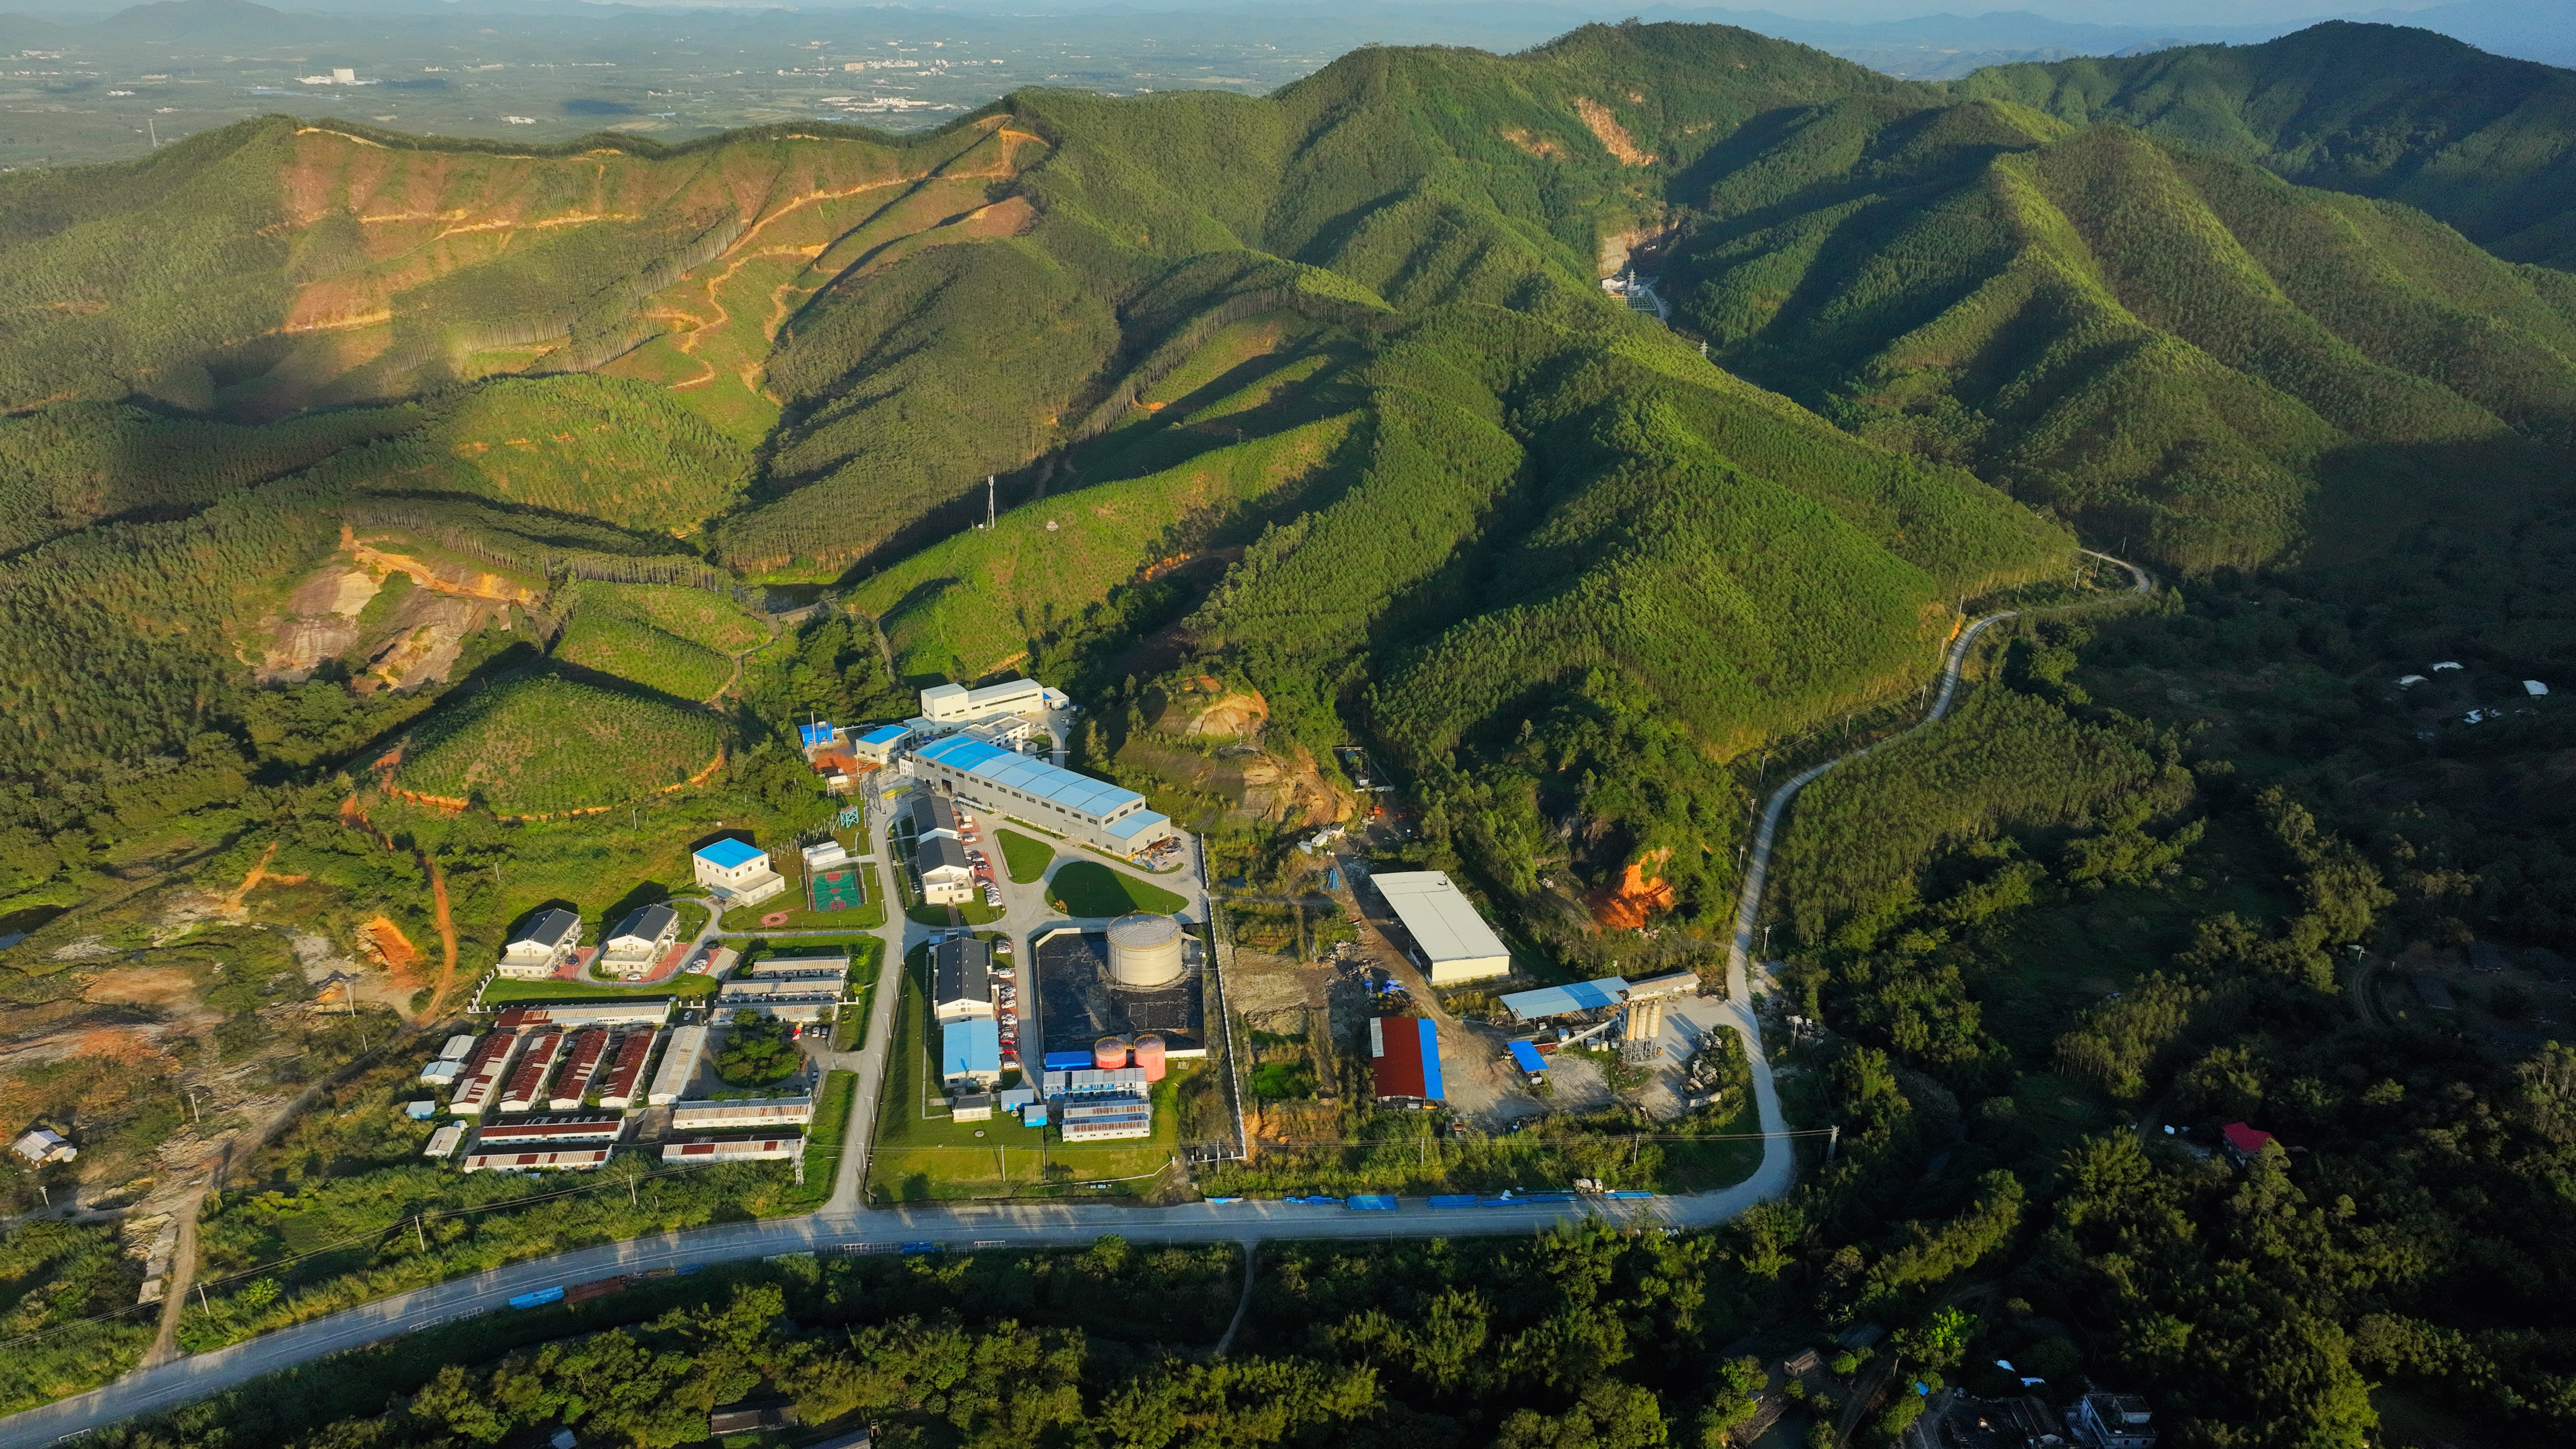
\includegraphics[width=\textwidth]{images/juno/juno_outside.jpg}
  \end{subfigure}
  \caption{\textbf{On the left:} Location of the JUNO experiment and its reactor sources in southern china. \textbf{On the right:} Aerial view of the experimental site}
\end{figure}

For this JUNO will measure the electronic anti-neutrinos ($\bar{\nu}_e$) flux coming from the nuclear reactors of Taishan, Yangjiang, for a total power of 26.6 GW$_{th}$, and the Daya Bay power plant to a lesser extent. Details about the power plants and there expected flux of $\bar{\nu}_e$ can be found in the table \ref{tab:power_plants}.
The distance of 53 km has been specifically chosen to maximize the disappearance probability of the $\bar{\nu}_e$.

\section{Neutrinos physics in JUNO}

Even if JUNO design (section \ref{sec:juno_detector})  was optimized for the measurement of the NMO, its large detection volume, excellent energy resolution and background level and understanding make it also an excellent detector to measure the flux coming from other neutrino sources. Thus the scientific program of JUNO extends way over reactor antineutrinos. The following section is an overview of the different physics topic JUNO will contribute in the coming years.

\subsection{Reactor neutrino oscillation for NMO and precise measurements}
\label{sec:nom_precise_measurement}
Previous works \cite{zhan_determination_2008,  zhan_experimental_2009} shows that oscillation parameters and the NMO can be observed by looking at the $\bnue$ disappearance spectrum coming from medium baseline nuclear reactor. This disappearance probability can be expressed as \cite{an_neutrino_2016} :
\begin{equation*}
  P(\bnue \rightarrow \bnue) = 1 - \sin^2 2\theta_{12} c^4_{13} \sin^2 \frac{\Delta m^2_{21}L}{4E} - \sin^2 2\theta_{13} \bigg[ c_{12}^2 \sin^2 \frac{\Delta m_{31}^2 L}{4E} + s^2_{12} \sin^2 \frac{\Delta m_{32}^2 L}{4E} \bigg]
\end{equation*}
Where $s_{ij} = \sin \theta_{ij}$, $c_{ij} = \cos \theta_{ij}$, $E$ is the $\bnue$ energy and $L$ is the baseline.
We can see the sensitivity to the NMO in the dependency to $\Delta m_{32}^2$ and $\Delta m^2_{31}$ causing a phase shift of the spectrum as we can see in the figure \ref{fig:juno-spectrum-oscillation}.
By carefully fitting this spectrum, one can extract the NMO and the oscillation parameters. The fit is reviewed in more details in the section \ref{sec:Fit}.
\begin{figure}
  \centering
  \includegraphics[height=8cm]{images/juno/Spectrum-OscillationsOnly_dm2_31.png}
  \caption{Expected number of neutrinos event per MeV in JUNO after 6 years of data taking. The black curve shows the flux if there was no oscillation. The light gray curve shows the oscillation if only the solar terms are taken in account ($\theta_{12}$, $\Delta m_{21}^2$). The blue and red curve shows the spectrum in the case of, respectively, NO and IO. The dependency of the oscillation to the different parameters are schematized by the double sided arrows. We can see the NMO sensitivity by looking at the fine phase shift between the red and the blue curve.}
  \label{fig:juno-spectrum-oscillation}
\end{figure}
To reach the desired sensitivity, JUNO must meet multiple requirements but most notably:
\begin{enumerate}
  \item An energy resolution of $3\%/\sqrt{E\mathrm{(MeV)}}$ to be able to distinguish the fine structure of the fast oscillation.
  \item An energy precision of 1\% in order to not err on the location of the oscillation pattern.
  \item A baseline of 53 $\pm$ 0.5 km to maximise the $\bar{\nu}_e$ oscillation probability.
  \item At least $\approx$ 100,000 events to limit the spectrum distortion dur to statistical uncertainties.
\end{enumerate}

\subsubsection{$\bar{\nu}_e$ flux coming from nuclear power plants}

To get such high measurements precision, it is necessary to have a very good understanding of the sources characteristics. For its NMO and precise measurement studies, JUNO will observe the energy spectrum of neutrinos coming from the nuclear power plants Taishan and Yangjiang's cores, located at 53 km of the detector to maximise the disappearance probability of the $\bar{\nu}_e$.

\begin{table}[ht]
  \centering
  \begin{tabular}{l c c c c}
    \hline
    Reactor & Power (GW$_{th}$) & Baseline (km) & IBD Rate (day$^{-1}$) & Relative Flux (\%) \\
    \hline
    Taishan    & 9.2  & 52.71 & 15.1 & 32.1 \\
    $~$ Core 1 & 4.6  & 52.77 & 7.5  & 16.0 \\
    $~$ Core 2 & 4.6  & 52.64 & 7.6  & 16.1 \\
    Yangjiang  & 17.4 & 52.46 & 29.0 & 61.5 \\
    $~$ Core 1 & 2.9  & 52.74 & 4.8  & 10.1 \\
    $~$ Core 2 & 2.9  & 52.82 & 4.7  & 10.1 \\
    $~$ Core 3 & 2.9  & 52.41 & 4.8  & 10.3 \\
    $~$ Core 4 & 2.9  & 52.49 & 4.8  & 10.2 \\
    $~$ Core 5 & 2.9  & 52.11 & 4.9  & 10.4 \\
    $~$ Core 6 & 2.9  & 52.19 & 4.9  & 10.4 \\
    Daya Bay   & 17.4 & 215   & 3.0  & 6.4  \\
    \hline
  \end{tabular}
  \caption{Characteristics of the nuclear power plants observed by JUNO. The IBD rate are estimated from the baselines, the reactors full thermal power, selection efficiency and the current knowledge of the oscillation parameters}
  \label{tab:power_plants}
\end{table}

The $\bar{\nu}_e$ coming from reactors are emitted from $\beta$-decay of unstable fission fragments. The Taishan and Yangjiang reactors are pressurised water reactor (PWR), the same type as Daya Bay. In those type of reactor more the 99.7 \% and $\bar{\nu}_e$ are produced by the fissions of four fuel isotopes $^{235}$U, $^{238}$U, $^{239}$Pu and $^{241}$Pu. The neutrino flux per fission of each isotope is determined by the inversion of the measured $\beta$ spectra of fission product \cite{hahn_antineutrino_1989, mueller_improved_2011, von_feilitzsch_experimental_1982, schreckenbach_determination_1985, huber_determination_2011} or by calculation using the nuclear databases \cite{vogel_reactor_1981, dwyer_spectral_2015}. The neutrino flux coming from a reactor at a time $t$ can be predicted using
\begin{equation}
  \phi(E_\nu, t)_r = \frac{W_{th}(t)}{\sum_i f_i(t) e_i} \sum_i f_i(t) S_i(E_\nu)
\end{equation}
where $W_{th}(t)$ is the thermal power of the reactor, $f_i(t)$ is the fraction fission of the $i$th isotope, $e_i$ its thermal energy released in each fission and $S_i(e_\nu)$ the neutrino flux per fission for this isotope. Using this method, the flux uncertainty is expected to be of an order of 2-3 \% \cite{juno_collaboration_sub-percent_2022}.

In addition to those prediction, a satellite experiment named TAO\cite{juno_collaboration_tao_2020} will be setup near the reactor core Taishan-1 to measure with an energy resolution of 2\% at 1 MeV the neutrino flux coming from the core. It will help identifying unknown fine structure and give more insight on the $\bar{\nu}_e$ flux coming from this reactor.

One  the open issue about reactor anti-neutrinos flux is the so-called neutrino anomaly \cite{mention_reactor_2011}, an unexpected surplus of neutrino emission in the spectra around 5 MeV.
Multiples scientists are trying to explain this surplus by advanced recalculation of the nuclei model during beta decay \cite{kopeikin_reevaluating_2021, letourneau_origin_2023} but no consensus on this issue has been reached yet.

\subsubsection{Background in the neutrinos reactor spectrum}

Considering the close reactor neutrinos flux as the main signal, the signals that are considered as background are:
\begin{itemize}
  \item The geoneutrinos producing background in the 0.511 $\sim$ 2.7 MeV region.
  \item The neutrinos coming from the other nuclear reactors around Earth.
\end{itemize}
In addition to all those physics signal, non-neutrinos signal that would mimic an IBD will also be present. It is composed of:
\begin{itemize}
  \item The signal coming from radioactive decay ($\alpha, ~ \gamma, ~ \beta$) from natural radioactive isotopes in the material of the detector.
  \item Cosmogenic event such as fast neutrons and activated isotopes induced by muons passing through the detector, most notably the spallation on $^{12}$C.
\end{itemize}
All those events represent a non-negligeable part of the spectrum as shown in figure \ref{fig:spectrum_with_background}.

\begin{figure}[ht]
  \centering
  \includegraphics[height=6cm]{images/juno/spectrum_with_background.png}
  \caption{Expected visible energy spectrum measured with the LPMT system with (grey) and without (black) backgrounds. The background amount for about 7\% of the IBD candidate and are mostly localized below 3 MeV \cite{juno_collaboration_sub-percent_2022}}
  \label{fig:spectrum_with_background}
\end{figure}


\subsubsection{Identification of the mass ordering}

To identify the mass ordering, we fit the neutrino energy spectrum under the two hypothesis of NO and IO. Those two fit give us two $\chi^2$, respectively $\chi^2_{NO}$ and $\chi^2_{IO}$. By computing the difference $\Delta \chi ^2 = \chi^2_{NO} - \chi^2_{IO}$ we can determine the most probable mass ordering: NO if $\Delta \chi^2 > 0$ and IO if $\Delta \chi^2 < 0$. Current studies shows that the expected sensitivity the mass ordering would be of $3.4 \sigma$ after 6 years of data taking in nominal setup\cite{an_neutrino_2016}. More detailed explanations about the fitting procedure can be found in the section \ref{sec:Fit}.

\subsubsection{Precise measurement of the oscillations parameters}

The oscillations parameters $\theta_{12}$, $\theta_{13}$, $\Delta m^2_{21}$, $\Delta m^2_{31}$ are free parameters in the fit of the oscillation spectrum. The precision on those parameters have been estimated and are shown in table \ref{tab:juno-param-precision}. Wee see that for $\theta_{12}$, $\Delta m^2_{21}$, $\Delta m^2_{31}$, precision at 6 years is better than the reference precision by an order of magnitude \cite{juno_collaboration_sub-percent_2022}


\begin{table}[ht]
  \centering
  \begin{tabular}{l | c c c c c}
    \hline
    & Central Value & PDG 2020 & 100 days & 6 years & 20 years \\
    \hline
    $\Delta m^2_{31} (\times 10^{-3} \mathrm{eV}^2)$ & 2.5283  & $\pm 0.034 ~ (1.3\%)$  & $\pm 0.021 ~ (0.8\%)$  & $\pm 0.0047 (0.2\%)$  & $\pm 0.0029 (0.1\%)$ \\
    $\Delta m^2_{21} (\times 10^{-3} \mathrm{eV}^2)$ & 7.53    & $\pm 0.18 ~ (2.4\%)$   & $\pm 0.074 ~ (1.0\%)$  & $\pm 0.024 (0.3\%)$   & $\pm 0.017  (0.2\%)$ \\
    $\sin ^2 \theta_{12}$                            & 0.307   & $\pm 0.013 ~ (4.2\%)$  & $\pm 0.0058 ~ (1.9\%)$ & $\pm 0.0016 (0.5\%)$  & $\pm 0.0010 (0.3\%)$ \\
    $\sin ^2 \theta_{13}$                            & 0.0218  & $\pm 0.0007 ~ (3.2\%)$ & $\pm 0.010 ~ (47.9\%)$ & $\pm 0.0026 (12.1\%)$ & $\pm 0.0016 (7.3\%)$ \\
    \hline
  \end{tabular}
  \caption{A summary of precision levels fir the oscillation parameters. The reference value (PDG 2020 \cite{particle_data_group_review_2020}) is compared with 100 days, 6 years and 20 years of JUNO data taking.}
  \label{tab:juno-param-precision}
\end{table}

\subsection{Other physics}

While the design of JUNO is tailored to measure $\bar{\nu}_e$ coming from nuclear reactor, JUNO will be able to detect neutrinos coming from other sources thus allowing for a wide range of physics studies as detailed in the table \ref{tab:signal} and in the following sub-sections.

\begin{table}[ht]
\begin{center}
  \begin{tabular}{|c|c|c|c|}
    \hline Research & Expected signal & Energy region & Major backgrounds \\
    \hline Reactor antineutrino & 60 IBDs/day & 0–12 MeV  & Radioactivity, cosmic muon \\
    Supernova burst & 5000 IBDs at 10 kpc & 0–80 MeV & Negligible \\
                    & 2300 elastic scattering  & &  \\
    DSNB (w/o PSD) & 2–4 IBDs/year & 10–40 MeV & Atmospheric $\nu$ \\
    Solar neutrino & hundreds per year for $^8$B & 0–16 MeV & Radioactivity \\
    Atmospheric neutrino & hundreds per year & 0.1–100 GeV  & Negligible \\
    Geoneutrino &  $\approx 400$ per year & 0–3 MeV & Reactor $\nu$ \\
    \hline
  \end{tabular}
  \caption{Detectable neutrino signal in JUNO and the expected signal rates and major background sources}
  \label{tab:signal}
\end{center}
\end{table}


\subsubsection{Geoneutrinos}

Geoneutrinos designate the antineutrinos coming from the decay of long-lived radioactive elements inside the Earth. The 1.8 MeV threshold necessary for the IBD makes it possible to measure geoneutrinos from $^{238}$U and $^{232}$Th decay chains. The studies of geoneutrinos can help refine the Earth crust models but is also necessary to characterise their signal, as they are a background to the mass ordering and oscillations parameters studies.

\subsubsection{Atmospheric neutrinos}

Atmospheric neutrinos are neutrinos originating from the decay of $\pi$ and $K$ particles that are produced in extensive air showers initiated by the interactions of cosmic rays with the Earth atmosphere. Earth is mostly transparent to neutrinos below the PeV energy, thus JUNO will be able to see neutrinos coming from all directions. Their baseline range is large (15km $\sim$ 13000km), they can have energy between 0.1 GeV and 10 TeV and will contain all neutrino and antineutrinos flavour. Their studies is complementary to the reactor antineutrinos and can help refine the constraints on the NMO \cite{an_neutrino_2016}.

\subsubsection{Supernovae burst neutrinos}

Neutrinos are crucial component during all stages of stellar collapse and explosion. Detection of neutrinos coming for core collapse supernovae will provide us important informations on the mechanisms at play in those events.
Thanks to its 20 kt LS, JUNO has excellent capabilities to detect all flavour of the $\mathcal{O}$(10 MeV) postshock neutrinos, and using neutrinos of the $\mathcal{O}$(1 MeV) will give informations about the pre-supernovae neutrinos. All those informations will allow to disentangle between the multiple hydro-dynamic models that are currently used to describe the different stage of core-collapse supernovae.

\subsubsection{Diffuse supernovae neutrinos background}

Core-collapse supernovae in our galaxy are rare events, but they frequently occur throughout the visible Universe sending burst of neutrinos in direction of the Earth. All those events contributes to a low background flux of low-energy neutrinos called the Diffuse Supernovae Neutrino Background (DSNB). Its flux and spectrum contains informations about the red-shift dependent supernovae rate, the average supernovae neutrino energy and the fraction of black-hole formation in core-collapse supernovae. Depending of the DSNB model, we can expect 2-4 IBD events per year in the energy range above the reactor $\bar{\nu}_e$ signal, which is competitive with the current Super-Kamiokande+Gadolinium phase \cite{collaboration_diffuse_2021}.

\subsubsection{Beyond standard model neutrinos interactions}

JUNO will also be able to probe for beyond standard model neutrinos interactions. After the main physics topics have been accomplished, JUNO could be upgraded to probe for neutrinoless beta decay ($0\nu\beta\beta$). The detection of such event would give critical informations about the nature of neutrinos, is it a majorana or a dirac particle. JUNO will also be able to probe for neutrinos that would come for the decay or annihilation of Dark Matter inside the sun and neutrinos from putative primordial black hole.
Through the unitary test of the mixing matrix, JUNO will be able to search for light sterile neutrinos.
Thanks to JUNO sensitivity, multiple other exotic can be performed on neutrino related beyond standard model interactions.


\section{The JUNO detector}
\label{sec:juno_detector}

The JUNO detector is a scintillator detector buried 693.35 meters under the ground (1800 meters water equivalent). It consist of Central Detector (CD), a water pool and a Top Tracker (TT) as showed in figure \ref{fig:juno-schema}
The CD is an acrylic vessel containing the 20 ktons of LS. It is supported by a stainless steel structure and is immersed in that water pool that is used as shielding from external radiation and as a cherenkov detector for the background. The top of the experiment is partially covered by the TT, a plastic scintillator detector which is use to detect the atmospheric muons background acting as veto detector.


The top of the experiment also host the LS purification system, a water purification system, a ventilation system to get rid of the potential radon in the air.
The CD is observed by two system of Photo-Multipliers Tubes (PMT). They are attached to the steel structure and their electronic readout is submersed near them. A third system of PMT is also installed on the structure but are facing outward of the CD, instrumenting the water to be cherenkov detector. The CD and the cherenkov detector are optically separated by Tyvek sheet. A chimney for LS filling and purification and for calibration operations connects the CD to the experimental hall from the top.

\begin{figure}[ht]
  \centering
  \begin{subfigure}[b]{0.45\textwidth}
    \centering
    \includegraphics[height=6cm]{images/juno/drawing_schema.png}
    \caption{Schematics view of the JUNO detector.}
    \label{fig:juno-schema}
  \end{subfigure}
  \hfill
  \begin{subfigure}[b]{0.45\textwidth}
    \centering
    \includegraphics[height=4cm]{images/juno/top_down_view.jpg}
    \caption{Top down view of the JUNO detector under construction}
  \end{subfigure}
\end{figure}

This section cover in details the different components of the detector and the detection systems.

\subsection{Principle of detection}

The CD will detect the neutrino and measure their energy mainly via an Inverse Beta Decay (IBD) interaction with proton (mainly $^{12}$C and H) in the LS:
\begin{equation*}
  \bar{\nu}_e + p \rightarrow n + e^+
\end{equation*}
Kinematics calculation shows that this interaction has an energy threshold for the $\bar{\nu}_e$ of $ (m_n + m_e - m_p ) \approx 1.806 ~ \mathrm{MeV}$ \cite{strumia_precise_2003} where $m_\lambda$ is the mass of the $\lambda$ particle.
This threshold make the experiment blind to very low energy neutrinos. The residual energy $E_{\nu} - 1.806 ~ \mathrm{MeV}$ is be distributed as kinetic energy between the positron and the neutron.
The energy of the emitted positron $E_e$ is given by \cite{strumia_precise_2003}
\begin{equation}
  E_e = \frac{(E_\nu - \delta)(1+\epsilon_\nu) + \epsilon_\nu \cos \theta \sqrt{(E_\nu - \delta)^2 + \kappa m_e^2}}{\kappa}
\end{equation}
where $\kappa = (1 + \epsilon_\nu)^2 - \epsilon_\nu^2 \cos^2 \theta \approx 1$, $\epsilon_\nu = \frac{E_\nu}{m_p} \ll 1$ and $\delta = \frac{m_n^2 - m_p^2 - m_e^2}{2m_p} \ll 1$.
We can see from this equation that the positron energy is strongly correlated to the neutrino energy.


The positron and the neutron will then propagate in the detection medium, the Liquid Scintillator (LS), loosing their kinetic energy by exciting the molecule of the LS (more details in section \ref{sec:LS}). Once stopped, the positron will annihilate with an electron from the medium producing two 511 KeV gamma. Those gamma will themselves interact with the LS, exciting it before being absorbed by photoelectrical effect. The neutron will be captured by an hydrogen, emitting a 2.2 MeV gamma in the process. This gamma will also deposit its energy before being absorbed by the LS.

\begin{figure}[ht]
  \centering
  \includegraphics[width=8cm]{images/juno/IDB-JUNO.png}
  \caption{Schematics of an IBD interaction in the central detector of JUNO}
  \label{fig:IBD}
\end{figure}

The scintillation photons have an UV frequency and will be captured by PMTs observing the CD. The analog signal of the PMTs digitized by the electronic is the signal of our experiment. The signal produced by the positron is subsequently called the prompt signal, and the signal coming from the neutron the delayed signal. This naming convention come from the fact that the positron will deposit its energy rather quickly (few ns) where the neutron will take a bit more time ($\sim$ 236 $\mu$s).

\subsection{Central Detector (CD)}
\label{sec:CD}

The central detector, composed of 20 ktons of Liquid Scintillator (LS), is the main part of JUNO. The LS is contained in a spherical acrylic vessel supported by a stainless steel structure. The CD and its structural support are submerged in a cylindrical water pool of 43.5m diameter and 44m height. We're confident that the water pool provide sufficient buffer protection in every direction against the rock radioactivity.
\subsubsection{Acrylic vessel}
The acrylic vessel is a spherical vessel of inner diameter of 35.4 m and a thickness of 120 mm. It is assembled from 265 acrylic panels, thermo bonded together. The acrylic recipes has been carefully tuned with extensive R\&D to ensure it does not include plasticizer and anti-UV material that would stop the scintillation photons.
Those panels requires to be pure of radioactive materials to not cause background. Current setup where the acrylic panels are molded in cleanrooms of class 10000, let us reach a uranium and thorium contamination of <0.5 ppt. The molding and thermoforming processes is optimized to increase the assemblage transparency in water to >96\%. The acrylic vessel is supported by a stainless steel structure via supporting node (fig \ref{fig:sup_node}). The structure and the nodes are designed to be resilient to natural catastrophic events such as earthquake and can support many times the effective load of the acrylic vessel.

\begin{figure}[ht]
  \centering
  \includegraphics[height=4cm]{images/juno/node_b.png}
  \caption{Schematics of the supporting node for the acrylic vessel}
  \label{fig:sup_node}
\end{figure}

\subsubsection{Liquid scintillator}
\label{sec:LS}

The Liquid Scintillator (LS) has a similar recipe as the one used in Daya Bay \cite{bay_optimization_2020} but without gadolinium doping. It is made of three components, necessary to shift the wavelength of emitted photons to prevent their reabsorption:
\begin{enumerate}
  \item The detection medium, the \textit{linear alkylbenzene} (LAB). Selected because of its excellent transparency, high flash point, low chemical reactivity and good light yield. Accounting for $\sim 98\%$ of the LS, it is the main component with which ionizing particles and gamma interact. Charged particles will collide with its electronic cloud transferring energy to the molecules, gamma will interact via compton effect with the electronic cloud before finally be absorbed via photoelectric effect.
  \item The second component of the LS is the \textit{2,5-diphenyloxazole} (PPO). A fraction of the excitation energy of the LAB is transferred to the PPO, mainly via non radiative process \cite{birks_chapter_1964}. The PPO molecules de-excites in the same way, transferring their energy to the bis-MSB. The PPO makes for $~1.5$ \% of the LS.
  \item The last component is the \textit{p-bis(o-methylstyryl)-benzene} (bis-MSB). Once excited by the PPO, it will emit photon with an average wavelength of $\sim430$ nm (full spectrum in figure \ref{fig:LS_spectrum_and_PMT_sensitivity}) that can be detected by our photo-multipliers systems. It amount for $\sim 0.5$\% of the LS.
\end{enumerate}

\begin{figure}[ht]
  \centering
  \begin{subfigure}[b]{0.48\textwidth}
    \centering
    \includegraphics[height=5cm]{images/juno/LS_spectrum.png}
  \end{subfigure}
  \hfill
  \begin{subfigure}[b]{0.48\textwidth}
    \centering
    \includegraphics[height=5cm]{images/juno/LPMT_efficiency.png}
  \end{subfigure}
  \caption{\textbf{On the left:} Quantum efficiency (QE) and emission spectrum of the LAB and the bis-MSB \cite{bay_optimization_2020}. \textbf{On the right:} Sensitivity of the Hamamatsu LPMT depending on the wavelength of the incident photons \cite{noauthor_photomultiplier_nodate}.}
  \label{fig:LS_spectrum_and_PMT_sensitivity}
\end{figure}

This formula has been optimized using dedicated studies with a Daya Bay detector \cite{bay_optimization_2020, zhang_complete_2020} to reach the requirements for the JUNO experiment:
\begin{itemize}
  \item A light yield / MeV of the amount of $10^4$ photons to maximize the statistic in the energy measurement.
  \item An attenuation length comparable to the size of the detector to prevent losing photons during their propagation in the LS. The final attenuation length is 25.8m \cite{yang_light_2017} to compare with the CD diameter of 35.4m.
  \item Uranium/Thorium radiopurity to prevent background signal. The reactor neutrino program require a contamination fraction $F<10^{-15}$ while the solar neutrino program require $F<10^{-17}$.
\end{itemize}

The LS will frequently be purified and tested in the Online Scintillator Internal Radioactivity Investigation System (OSIRIS) \cite{juno_collaboration_design_2021} to ensure that the requirements are kept during the lifetime of the experiment.

\subsubsection{Large Photo-Multipliers Tubes(LPMTs)}
\label{sec:LPMT}

The scintillation light produced by the LS is then collected by Photo-Multipliers Tubes (PMT) that transform the incoming photon into an electric signal. As described in figure \ref{fig:pmt-schem}, the incident photons interact with the photocatode via photoelectric effect producing an electron called a Photo-Electron (PE). This PE is then focused on the dynodes where the high voltage will allow it to be multiplied. After multiple amplification the resulting charge - in coulomb [C] - is collected by the anode and the resulting electric signal can be digitalized by the readout electronics from which the charge and timing can be extracted.

\begin{figure}[ht]
  \centering
  \includegraphics[height=4cm]{images/juno/pmt_schematic.png}
  \caption{Schematic of a PMT}
  \label{fig:pmt-schem}
\end{figure}

The Large Photo-Multipliers Tubes (LPMT), used in the central detector and in the water pool, are 20-inch (50.8 cm) radius PMTs. $\sim 5000$ dynode-PMTs \cite{noauthor_photomultiplier_nodate} were produced by the Hamamatsu$^{\copyright}$ company and $\sim 15000$ Micro-Channel Plate (MCP) \cite{abusleme_mass_2022} by the NNVT$^{\copyright}$ company. This system is the one responsible for the energy measurement with a energy resolution of $3\%/\sqrt{E}$, resolution necessary for the mass ordering measurement. To reach this precision, the system is composed of 17612 PMTs quasi uniformly distributed over the detector for a coverage of 75.2\% reaching $\sim 1800$ PE/MeV or $\sim 2.3 \%$ resolution due to statistic, leaving $\sim 0.7\%$ for the systematic uncertainties.
To maintain the resolution over the lifetime of the experiment, JUNO require a failure rate < 1\% over 6 years.

The LPMTs electronic are divided in two parts. One "near", located underwater, in proximity of the LPMT to reduce the cable length between the PMT and early electronic. A second one, outside of the detector that is responsible for higher level analysis before sending the data to the DAQ.

The light yield per MeV induce that a LPMT can collect between 1 and 1000 PE per event, causing non linearity in the PMT response that need to be understood and calibrated, see section \ref{sec:calib} for more details.

\subsubsection{Small Photo-Multipliers Tubes (SPMTs)}
\label{sec:SPMT}

The Small PMT (SPMTs) system is made of 3-inch (7.62 cm) PMTs. They will be used in the CD as a secondary detection system. Those 25600 SPMTs will observe the same events as the LPMTs, thus sharing the physics and detector systematics up until the photon conversion. With a detector coverage of 2.7\%, this system will collect $\sim 43$ PE/MeV for a final energy resolution of $\sim 17\%$. This resolution is not enough to measure the NMO, $\theta_{13}$, $\Delta m^2_{31}$ but will be sufficient to independently measure $\theta_{12}$ and $\Delta m^2_{21}$.

Due to the low PE rate, SPMTs will be running in photo-counting mode in the reactor range thus will be insensitive to non-linearity effect. Also, due to their smaller size and electronics, SPMTs have a better timing resolutions than the LPMTs.
At higher energy range, like supernovae events, LPMTs will saturate where SPMTs due to their lower PE collection will to produce a reliable measure of the energy spectrum.

The Data Acquisition System (DAQ) is designed to support the event rate of IBD, background, dark noise and supplementary storage buffers are present in the LPMT electronics to withstand the event rate during supernovae burst.

\subsection{Veto detector}

The CD will be bathed in constant background noise coming from numerous sources : the radioactivity from surrounding rock and its own components or from the flux of cosmic muons. This background needs to be rejected to ensure the purity of the IBD spectrum. To prevent a big part of them, JUNO use two veto detector that will tag events as background before CD analysis.

\subsubsection{Cherenkov in water pool}

The Water Cherenkov Detector (WCD) is the instrumentalization of the water buffer around the CD. When high speed charged particles will pass through the water, they will produced cherenkov photons. The light will be collected by 2400 MCP LPMTs installed on the outer surface of the CD structure. The  muons veto strategy is based on a PMT multiplicity condition. WCD PMTs are grouped in ten zones: 5 in the top, 5 in the bottom. A veto is raised either when more than 19 PMTs are triggered in one zone or when two adjacent zones simultaneously trigger more than 13 PMTs. Using this trigger, we expect to reach a muon detection efficiency of 99.5\% while keeping the noise at reasonable level.

\subsubsection{Top tracker}
The JUNO Top Tracker (TT) is a plastic scintillator detector located on the top of the experiment (see figure \ref{fig:tt}). Made from plastic scintillator from OPERA \cite{acquafredda_opera_2009} layered horizontally in 3 layers on the top of the detector, the TT will be able to detect incoming atmospheric muons.
With its coverage, about 1/3 of the of all atmospheric muons that passing through the CD will also pass through the 3 layer of the detector. While it does not cover the majority of the CD, the TT is particularly effective to detect muons coming through the filling chimney region which might present difficulties from the other subsystems in some classes of events.
\begin{figure}[ht]
  \centering
  \includegraphics[height=5cm]{images/juno/Global_TT_01.png}
  \caption{The JUNO top tracker}
  \label{fig:tt}
\end{figure}

\section{Calibration strategy}
\label{sec:calib}

The calibration is a crucial part of the JUNO experiment. Because we are looking at civil reactor neutrino it might be impossible to run measurement without signal, it would need to shut down every reactor from the Taishan and Yangjiang power plants which is realistically impossible. Because of this continuous rate, low frequency signal event, we need high frequency, recognisable sources in the energy range of interest : [0-12] MeV for the positron signal and 2.2 MeV for the neutron capture.
It is expected that the CD response will be different depending on the type of particle, due to the interaction with LS, the position on the event and the optical response of the acrylic sphere (see section \ref{sec:reco}).
We also expect a non-linear energy response of the CD due to the LS properties \cite{bay_optimization_2020} but also due to the saturation of the LPMTs system when collecting a large amount of PE \cite{han_dual_2021}.

\subsection{Energy scale calibration}

While electrons and positrons sources would be ideal, for a large LS detector thin-walled electrons or positrons sources could lead to leakage of radionucleides causing radioactive contamination. Instead, we consider gamma sources in the range of the prompt energy of IBDs. The sources are reported in table \ref{tab:calib_source}.

\begin{table}[ht]
  \centering
  \begin{tabular}{|c|c|c|}
    \hline
    Sources / Processes & Type & Radiation \\
    \hline
    $^{137}$Cs          & $\gamma$ & 0.0662 MeV \\
    $^{54}$Mn           & $\gamma$ & 0.835 MeV \\
    $^{60}$Co           & $\gamma$ & 1.173 + 1.333 MeV \\
    $^{40}$K            & $\gamma$ & 1.461 MeV \\
    $^{68}$Ge           & $e^{+}$  &  annihilation 0.511 + 0.511 MeV \\
    $^{241}$Am-Be       & $n,\gamma$ & neutron + 4.43 MeV (${12}$C*) \\
    $^{241}$Am-$^{13}$C & $n,\gamma$ & neutron + 6.13 MeV (${16}$O*) \\
    $(n, \gamma)p$      & $\gamma$ & 2.22 MeV \\
    $(n, \gamma)^{12}$C & $\gamma$ & 4.94 MeV or 3.68 + 1.26 MeV \\
    \hline
  \end{tabular}
  \caption{List of sources and their process considered for the energy scale calibration}
  \label{tab:calib_source}
\end{table}

For the $^{68}$Ge source, it will decay in $^{68}$Ga via electron capture, which will itself $\beta^+$ decay into $^{68}$Zn. The positrons will be absorbed by the enclosure so only the annihilation gamma will be released. In addition, $(\alpha, n)$ sources like $^{241}$Am-Be and $^{241}$Am-$^{13}$C are used to provide both high energy gamma and neutrons, which will later be captured in the LS producing the 2.2 MeV gamma.

From this calibration we call $E_{vis}$ the "visible energy" that is reconstructed by our current algorithms and we compare it to the true energy deposited by the calibration source. The results shown in figure \ref{fig:nl} show the expected response of the detector from calibration sources. The non-linearity is clearly visible from the $E_{vis} / E_{true}$ shape. See \cite{juno_collaboration_calibration_2021} for more details.

\begin{figure}[ht]
  \centering
  \begin{subfigure}[b]{0.24\textwidth}
    \centering
    \includegraphics[width=\textwidth]{images/juno/gamma_nl.png}
    \caption{Gamma non-linearity}
    \label{fig:nl:gamma}
  \end{subfigure}
  \begin{subfigure}[b]{0.37\textwidth}
    \centering
    \includegraphics[width=\textwidth]{images/juno/boron_nl.png}
    \caption{Boron non-spectrum}
    \label{fig:nl:boron}
  \end{subfigure}
  \begin{subfigure}[b]{0.37\textwidth}
    \centering
    \includegraphics[width=\textwidth]{images/juno/e-_nl.png}
    \caption{Electron non-linearity}
    \label{fig:nl:electron}
  \end{subfigure}
  \caption{Fitted and simulated non linearity of gamma, electron sources and from the $^{12}$B spectrum. Black points are simulated data. Red curves are the best fits}
  \label{fig:nl}
\end{figure}

\subsection{Calibration system}

The non-uniformity due to the event position in the detector (more details in section \ref{sec:reco}) will be studied using multiples systems that are schematized in figure \ref{fig:calib}. They allow to position sources at different location in the CD.

\begin{itemize}
  \item For a one-dimension vertical calibration, the Automatic Calibration Unit (ACU) will be able to deploy multiple radioactive sources or a pulse laser diffuser ball along the central axis of the CD through the top chimney. The source position precision is less than 1cm.
  \item For off-axis calibration, a calibration source attached to a Cable Loop System (CLS) can be moved on a vertical half-plane by adjusting the length of two connection cable. Two set of CSL will be deployed to provide a 79\% effective coverage of a vertical plane.
  \item A Guiding Tube (GT) will surround the CD to calibrate the non-uniformity of the response at the edge of the detector
  \item A Remotely Operated under-LS Vehicle (ROV) can be deployed to desired location inside LS for a more precise and comprehensive calibration. The ROV will also be equipped with a camera for inspection of the CD.
\end{itemize}

\begin{figure}[ht]
  \centering
  \includegraphics[height=6cm]{images/juno/calib.png}
  \caption{Overview of the calibration system}
  \label{fig:calib}
\end{figure}

The preliminary calibration program is depicted in table \ref{tab:calib_prog}.

\begin{table}[ht]
  \centering
  \begin{tabular}{c c c c}
    \hline
    Program & Purpose & System & Duration [min] \\
    \hline
    Weekly calibration & Neutron (Am-C) & ACU & 63 \\
                       & Laser & ACU & 78  \\
                       \hline
    Monthly calibration & Neutron (Am-C) & ACU & 120 \\
                        & Laser  & ACU  & 147 \\
                        & Neutron (Am-C) & CLS & 333 \\
                        & Neutron (Am-C) & GT  & 73  \\
                        \hline
    Comprehensive calibration & Neutron (Am-C) & ACU, CLS and GT & 1942 \\
                              & Neutron (Am-Be) & ACU & 75 \\
                              & Laser & ACU & 391 \\
                              & $^{68}$Ge & ACU & 75 \\
                              & $^{137}$Cs & ACU & 75 \\
                              & $^{54}$Mn & ACU & 75 \\
                              & $^{60}$Co & ACU & 75 \\
                              & $^{40}$K & ACU & 158 \\
    \hline
  \end{tabular}
  \caption{Calibration program of the JUNO experiment}
  \label{tab:calib_prog}
\end{table}

\section{Software}
\label{sec:software}

The simulation, reconstruction and analysis algorithms are all packaged in the JUNO software, subsequently called the software.
It is composed of multiple components integrated in the SNiPER \cite{lin_application_2017} framework:

\begin{itemize}
  \item Various primary particles simulators for the different kind of events, background and calibration sources.
  \item A Geant4 \cite{agostinelli_geant4simulation_2003, allison_geant4_2006, allison_recent_2016} Monte Carlo (MC) simulation containing the detectors geometries, a custom optical model for the LS and the supporting structures of the detectors. The Geant4 simulation integrate all relevant physics process for JUNO, validated by the collaboration. This step of the simulation is commonly called \textit{Detsim} and compute up to the production of photo-electrons in the PMTs. The optics properties of the different materials and detector components have been measured beforehand to be used to define the material and surfaces in the simulation.
  \item An electronic simulation, simulating the response waveform of the PMTs, tracking it through the digitization process, accounting for effects such as non-linearity, dark noise, Time Transit Spread (TTS), pre-pulsing, after-pulsing and ringing if the waveform. It's also the step handling the event triggers and mixing. This step is commonly referenced as \textit{Elecsim}.
  \item A waveform reconstruction where the digitized waveform are filtered to remove high-frequency white noise and then deconvoluted to yield time and charge informations of the photons hits on the PMTs. This step is commonly referenced as \textit{Calib}.
  \item The charge and time informations are used by reconstruction algorithms to reconstruct the interaction vertex and the deposited energy. This step is commonly reported as \textit{Reco}. See section \ref{sec:reco} for more details on the reconstruction.
  \item Once the singular events are reconstructed, they go through event pairing and classification to select IBD events. This step is named Event Classification.
  \item The purified signal is then analysed by the analysis framework which depend of the physics topic of interest.
\end{itemize}

The steps Reco and Event Classification are divided into two category of algorithm. Fast but less accurate algorithms that are running during the data taking designated as the \textit{Online} algorithms. Those algorithm are used to take the decision to save the event on tape or to throw it away. More accurate algorithms that run on batch of events designated \textit{Offline} algorithms. They are used for the physics analysis. The Offline Reco will be one of the main topic of interest for this thesis.

\section{State of the art of the Offline IBD reconstruction in JUNO}
\label{sec:reco}

The main reconstruction method currently run in JUNO is a data-driven method based on a likelihood maximization \cite{wu_new_2019, huang_improving_2021} using only the LPMTs. The first step is to reconstruct the interaction vertex from which the energy reconstruction is dependent. It is also necessary for event pairing and classification.

\subsection{Interaction vertex reconstruction}

To start the likelihood maximization, a rough estimation of the vertex and of the event timing is needed. We start by estimating the vertex position using a charge based algorithm.

\subsubsection{Charge based algorithm}

The charge-based algorithm is basically base on the charge-weighted average of the PMT position.

\begin{align}
  \vec{r}_{cb} = a\cdot\frac{\sum_i q_i \cdot \vec{r}_i}{\sum_i q_i}
\end{align}

Where $q_i$ is the reconstructed charge of the pulse of the $i$th PMT and $\vec{r}_i$ is its position. $\vec{r}_0$ is the reconstructed interaction position. $a$ is a scale factor introduced because a weighted average over a 3D sphere is inherently biased. Using calibration we can estimate $a \approx 1.3$ \cite{li_event_2021}. The results in figure \ref{fig:rec:cbary} shows that the reconstruction is biased from around 15m and further. This is due to the phenomena called ``total reflection area'' or TR Area.

As depicted in the figure \ref{fig:rec:refl} the optical photons, given that they have a sufficiently large incidence angle, can be deviated of their trajectories when passing through the interfaces LS-acrylic and water-acrylic due to the optical index difference. This cause photons to be lost or to be detected by PMT further than anticipated if we consider their rectilinear trajectories. This cause the charge barycenter the be located closer to the center than the event really is.

\begin{figure}[ht]
  \begin{subfigure}[t]{0.48\textwidth}
    \centering
    \includegraphics[height=6cm]{images/juno/reco/Reflexion_scenarii.jpg}
    \caption{Illustration of the different optical photons reflection scenarios. \textbf{1} is the reflection of the photon at the interface LS-acrylic or acrylic-water. \textbf{2} is the transmission of the photons through the interfaces. \textbf{3} is the conduction of the photon in the acrylic.}
    \label{fig:rec:refl}
  \end{subfigure}
  \hfill
  \begin{subfigure}[t]{0.48\textwidth}
    \centering
    \includegraphics[height=6cm]{images/juno/reco/charge_barycenter.png}
    \caption{Heatmap of $R_{rec}$ and $R_{rec} - R_{true}$ as a function of $R_{true}$ for 4MeV prompt signals uniformly distributed in the detector calculated by the charge based algorithm}
    \label{fig:rec:cbary}
  \end{subfigure}
  \caption{}
\end{figure}

It is to be noted that charge based algorithm, in addition to be biased near the edge of the detector, does not provide any information about the timing of the event. Therefore, a time based algorithm needs to be introduced to provide initial values.

\subsubsection{Time based algorithm}

The time based algorithm use the distribution of the time of flight corrections $\Delta t$ (Eq \ref{eq:rec:tof_corr}) of an event to reconstruct its vertex and $t_0$. It follow the following iterations:

\begin{enumerate}
  \item Use the charge based algorithm to get an initial vertex to start the iteration.

  \item \label{alg:rec:tba} Calculate the time of flight correction for the $i$th PMT using \begin{equation}
      \label{eq:rec:tof_corr}
      \Delta t_i (j) = t_i - \mathrm{tof}_i (j)
    \end{equation}
    where $j$ is the iteration step, $t_i$ is the timing of the $i$th PMT, and $\mathrm{tof}_i$ is the time-of-flight of the photon considering an rectilinear trajectory and an effective velocity in the LS and water (see \cite{li_event_2021} for detailed description of this effective velocity). Plot the $\Delta t$ distribution and label the peak position as $\Delta t^{\mathrm{peak}}$ (see fig \ref{fig:rec:delta_t_distrib}).

  \item Calculate a correction vector $\vec{\delta} [\vec{r}(j)]$ as \begin{equation}
      \vec{\delta} [\vec{r}(j)] = \frac{\sum_i \bigg(\frac{\Delta t(j) - \Delta t^{\mathrm{peak}}(j)}{\mathrm{tof}_i(j)} \bigg) \cdot (\vec{r}_0(j) - \vec{r}_i)}{N^{\mathrm{peak}}(j)}
    \end{equation}
    where $\vec{r}_0$ is the vertex position at the beginning of this iteration, $\vec{r}_i$ is the position of the $i$th PMT. To minimize the effect of scattering, dark noise and reflection, only the pulse happening in a time window (-10 ns, +5 ns) around $\Delta t^{\mathrm{peak}}$ are considered. $N^{\mathrm{peak}}$ is the number of PE collected in this time-window.

  \item if $\vec{\delta} [\vec{r}(j)] < 1 \mathrm{mm}$ or $j \geq 100$, stop the iteration. Otherwise $\vec{r}_0 (j + 1) = \vec{r}_0 (j) + \vec{\delta} [\vec{r}(j)]$ and go to step \ref{alg:rec:tba}.
\end{enumerate}

\begin{figure}
  \begin{subfigure}[t]{0.48\textwidth}
    \centering
    \includegraphics[width=\textwidth]{images/juno/reco/delta_t_peak_distrib.png}
    \caption{$\Delta t$ distribution at different iterations step $j$}
    \label{fig:rec:delta_t_distrib}
  \end{subfigure}
  \hfill
  \begin{subfigure}[t]{0.48\textwidth}
    \centering
    \includegraphics[width=\textwidth]{images/juno/reco/time_based_algorithm.png}
    \caption{Heatmap of $R_{rec}$ and $R_{rec} - R_{true}$ as a function of $R_{true}$ for 4MeV prompt signals uniformly distributed in the detector calculated by the time based algorithm}
    \label{fig:rec:time_based_results}
  \end{subfigure}
\end{figure}

However because the earliest arrival time is used, $t_i$ is related to the number photoelectrons $N_i^{\mathrm{pe}}$ detected by the PMT \cite{ranucci_analytical_1995, galbiati_time_2006, moszynski_status_1979}. To reduce bias in the vertex reconstruction, the following equation is used to correct $t_i$ into $t'_i$:
\begin{equation}
  t'_{i} = t_i - p_0 / \sqrt{N_i^{\mathrm{pe}}} - p_1 - p_2 / N_i^{\mathrm{pe}}
\end{equation}

The parameters $(p_0, p_1, p_2)$ were optimized to (9.42, 0.74, -4.60) for Hamamatsu PMTs and (41.31, -12.04, -20.02) for NNVT PMTs \cite{li_event_2021}. The results presented in figure \ref{fig:rec:time_based_results} shows that the time based algorithm provide a more accurate vertex and is unbiased even in the TR area. This results $(\vec{r}_0, t_0)$ is used as initial value for the likelihood algorithm.

\subsubsection{Time likelihood algorithm}

The time likelihood algorithm use the residual time expressed as follow
\begin{equation}
  \label{eq:rec:t_res}
  t_{\mathrm{res}}^i(\vec{r}_0, t_0) = t_i - \mathrm{tof}_i - t_0
\end{equation}

In a first order approximation, the scintillator time response Probability Density Function (PDF) can be described as the emission time profile of the scintillation photons, the Time Transit Spread (TTS) and the dark noise of the PMTs. The emission time profile $f(t_{\mathrm{res}})$ is described like
\begin{equation}
  f(t_{\mathrm{res}}) = \sum_k \frac{\rho_k}{\tau_k} e^{\frac{-t_{\mathrm{res}}}{\tau_k}}, ~ \sum_k \rho_k = 1
\end{equation}
as the sum of the $k$ component that emit light in the LS each one characterised by it's decay time $\tau_k$ and intensity fraction $\rho_k$. The TTS component is expressed as a gaussian convolution
\begin{equation}
  g(t_{\mathrm{res}}) = \frac{1}{\sqrt{2\pi}\sigma}e^{\frac{-(t_{\mathrm{res}} - \nu)^2}{2\sigma^2}} \cdot f(t_{\mathrm{res}})
\end{equation}
where $\sigma$ is the TTS of PMTs and $\nu$ is the average transit time. The dark noise is not correlated with any physical events and considered as constant rate over the time window considered $T$. By normalizing the dark noise probability $\epsilon(t_{\mathrm{res}})$ as $\int_T \epsilon(t_{\mathrm{res}}) dt_{\mathrm{res}} = \epsilon_{\mathrm{dn}}$ , it can be integrated in the PDF as
\begin{equation}
  \label{eq:juno:tim_like:dn}
  p(t_{\mathrm{res}}) = (1-\epsilon_{\mathrm{dn}}) \cdot g(t_{\mathrm{res}}) + \epsilon(t_{\mathrm{res}})
\end{equation}

The distribution of the residual time $t_{\mathrm{res}}$ of an event can then be compared to $p(t_{\mathrm{res}})$ and the best fitting vertex $\vec{r}_0$ and $t_0$ can be chosen by minimizing
\begin{equation}
  \mathcal{L}(\vec{r}_0, t_0) = - \mathrm{ln} \bigg(\prod_i p(t^i_{\mathrm{res}}) \bigg)
\end{equation}

The parameter of Eq. \ref{eq:juno:tim_like:dn} can be measured experimentally. The results shown in figure \ref{fig:rec:time_likelihood} used PDF from monte carlo simulation. The results shows that $R_{rec} - R_{true}$ is biased depending on the energy. While this could be corrected using calibration, another algorithm based on charge likelihood was developed to correct this problem.

\begin{figure}[ht]
  \centering
  \includegraphics[width=\linewidth]{images/juno/reco/time_likelihood_results.png}
  \caption{Bias of the reconstructed radius R (left), $\theta$ (middle) and $\phi$ (right) for multiple energies by the time likelihood algorithm}
  \label{fig:rec:time_likelihood}
\end{figure}


\subsubsection{Charge likelihood algorithm}

Similarly to the time likelihood algorithms that use a timing PDF, the charge likelihood algorithm use a PE PDF for each PMT depending on the energy and position of the event. With $\mu(\vec{r}_0, E)$ the mean expected number of PE detected by each PMT, the probability to observe $N_{pe}$ in a PMT follow a Poisson distribution. Thus
\begin{itemize}
  \item The probability to observe no hit ($N_{pe} = 0$) in the $j$th PMT is $P^{j}_{nohit} (\vec{r}_0, E) = e^{-\mu_j}$
  \item The probability to observe $N_{pe} \neq 0$ in the $i$th PMT is $P^{i}_{hit} (\vec{r}_0, E) = \frac{\mu^{N^i_{pe}} e^{-\mu_i}}{N^i_{pe}!}$
\end{itemize}

Therefore, the probability to observe a specific hit pattern can be expressed as
\begin{equation}
  P(\vec{r}_0, E) = \prod_j P^j_{nohit}(\vec{r}_0, E) \cdot \prod_i P^i_{hit}(\vec{r}_0, E)
\end{equation}

The best fit values of $\vec{R}_0$ and $E$ can then be calculated by minimizing the negative log-likelihood
\begin{equation}
  \label{eq:rec:charge_likelihood}
  \mathcal{L}(\vec{r}_0, E) = - \mathrm{ln}(P(\vec{r}_0,E))
\end{equation}

In principle, $\mu_i(\vec{r}_0, E)$ could be expressed
\begin{equation}
  \label{eq:rec:mu_i}
  \mu_i(\vec{r}_0, E) = Y \cdot \frac{\Omega(\vec{r}_0, r_i)}{4 \pi} \cdot \epsilon_i \cdot f(\theta_i) \cdot e^{-\sum_m \frac{d_m}{\zeta_m}}\cdot E + \delta_i
\end{equation}
where $Y$ is the energy scale factor, $\Omega(\vec{r}_0, r_i)$ is the solid angle of the $i$th PMT, $\epsilon_i$ is its detection efficiency, $f(\theta_i)$ its angular response, $\zeta_m$ is the attenuation length in the materials and $\delta_i$ the expected number of dark noise.

However Eq. \ref{eq:rec:mu_i} assume that the scintillation light yield is linear with energy and describe poorly the contribution of indirect light, shadow effect due to the supporting structure and the total reflection effects. The solution is to use data driven methods to produce the pdf by using the calibrations sources and position described in section \ref{sec:calib}. In the results presented in figures \ref{fig:rec:time_charge_results}, the PDF was produced using MC simulation and 29 specific calibrations position \cite{li_event_2021} along the Z-axis of the detector.
\begin{figure}[ht]
  \centering
  \begin{subfigure}[b]{0.48\linewidth}
    \centering
    \includegraphics[width=\textwidth]{images/juno/reco/charge_likelihood_res.png}
  \end{subfigure}
  \hfill
  \begin{subfigure}[b]{0.48\linewidth}
    \centering
    \includegraphics[width=\textwidth]{images/juno/reco/charge_likelihood_bias.png}
  \end{subfigure}
  \caption{\textbf{On the left:} Resolution of the reconstructed R as a function of the energy in the TR area ($R^3 > 4000 \mathrm{m}^3 \equiv R > 16 m$) by the charge and time likelihood algorithms. \textbf{On the right:} Bias of the reconstructed R in the TR area for different energies by the charge likelihood algorithm}
  \label{fig:rec:time_charge_results}
\end{figure}
We see that the charge likelihood algorithm show little bias in the TR area and a better resolution than the time likelihood. The figure \ref{fig:rec:all_class} shows the radial resolution of the different algorithm presented for this section, we can see the refinement at each step and that the charge likelihood yield the best results.

\begin{figure}[ht]
  \centering
  \includegraphics[height=6cm]{images/juno/reco/vertex_reco_classique.png}
  \caption{Radial resolution of the different vertex reconstruction algorithms as a function of the energy}
  \label{fig:rec:all_class}
\end{figure}

The charge based likelihood algorithms already give use some information on the energy as Eq. \ref{eq:rec:charge_likelihood} is minimized but the energy can be further refined as shown in the next section.


\subsection{Energy reconstruction}

As explained in section \ref{sec:nom_precise_measurement}, energy resolution is crucial for the NMO and oscillation parameters measurements. Thus the energy reconstruction algorithm should take into consideration as much detector effect as possible. The following method is a data driven method based on calibration samples inspired by the charge likelihood algorithm described above \cite{huang_data-driven_2023}.


\begin{figure}[ht]
  \centering
  \includegraphics[height=6cm]{images/juno/reco/energy_reco_vars.png}
  \caption{Definition of the variables used in the energy reconstruction}
  \label{fig:rec:energy_vars}
\end{figure}

\subsubsection{Charge estimation}

The most important element in the energy reconstruction is $\mu_i(\vec{r}_0, E)$ described in Eq. \ref{eq:rec:mu_i}. For realistic cases, we also need to take into account the electronics effect that were omitted in the previous section. Those effect will cause a charge smearing due to the uncertainties in the $N_{pe}$ reconstruction. Thus we define $\hat{\mu}^L(\vec{r}_0, E)$ which is the expected $N_{pe}/E$ in the whole detector for an event with visible energy $E_{vis}$ and position $\vec{r}_0$. The position of the event and PMTs are now defined using $(r, \theta, \theta_{pmt})$ as defined in figure \ref{fig:rec:energy_vars}.
\begin{equation}
  \hat{\mu}(r, \theta, \theta_{pmt}, E_{vis}) = \frac{1}{E_{vis}} \frac{1}{M} \sum_i^M\frac{\frac{\bar{q}_i}{\hat{Q}_i} - \mu_i^D}{\mathrm{DE}_i}, ~ \mu_i^D = \mathrm{DNR}_i \cdot L
\end{equation}
where $i$ runs over the PMTs with the same $\theta_{pmt}$, $\mathrm{DE}_i$ is the detection efficiency of the $i$th PMT. $\mu_i^D$ is the expected number of dark noise photoelectrons in the time window $L$. The time window have been optimized to $L = 280 ~ \mathrm{ns}$ \cite{huang_data-driven_2023}. $\bar{q}_i$ is the average recorded photoelectrons in the time window and $\hat{Q}_i$ is the expected average charge for 1 photoelectron. The $N_{pe}$ map is constructed following the procedure described in \cite{huang_improving_2021}.

\subsubsection{Time estimation}

The second important observable is the hit time of photons that was previously defined in Eq. \ref{eq:rec:t_res}. It is here refined as
\begin{equation}
  t_r = t_h - \mathrm{tof} - t_0 = t_{LS} + t_{TT}
\end{equation}
where $t_h$ is the time of hit, $t_{LS}$ is the scintillation time and $t_{TT}$ the transit time of PMTs that is described by a gaussian
\begin{equation}
  t_{TT} = \mathcal{N}(\overline{\mu_{TT} + t_{d}}, \sigma_{TT})
\end{equation}
where $\mu_{TT}$ is the mean transit time in PMTs, $\sigma_{TT}$ is the Transit Time Spread (TTS) of the PMTs and $t_{d}$ is the delay time in the electronics. The effective refraction index of the LS is also corrected to take into account the propagation distance in the detector.

The timing PDF $P_T(t_r | r,d,\mu_l,\mu_d,k)$ can now be generated using calibration sources \cite{huang_data-driven_2023}. This PDF describe the probability that the residual time of the first photon hit is in $[t_r, t_r + \delta]$ with $r$ the radius of the event vertex, $d = |\vec{r} - \vec{r}_{PMT}|$ the propagation distance, $\mu_l$ and $\mu_d$ the expected number of PE and dark noise in the electronic reading window and $k$ is the detected number of PE.

Now let denote $f(t, r, d)$ the probability density function of "photoelectron hit a time t" for an event happening at $r$ where the photons traveled the distance $d$ in the LS
\begin{equation}
  F(t, r, d) = \int_t^L f(t', r, d)dt'
\end{equation}
Based on the PDF for one photon $k=1$, one can define
\begin{equation}
  P^l_T(t|k=n) = I^l_n [f_l(t)F^{n-1}_l(t)]
\end{equation}
where the indicator $l$ means that the photons comes from the LS and $I^l_n$ a normalisation factor. To this pdf we add the probability to have photons coming from the dark noise indicated by the indicator $d$ using
\begin{equation}
  f_d(t) = 1 / L, ~ F_d(t) = 1 - \frac{t}{L}
\end{equation}
and so for the case where only one photon is detected by the PMT ($k=1$)
\begin{equation}
  P_T(t|\mu_l, \mu_d, k = 1) = I_1 [ P(1, \mu_l) P(0, \mu_d) f_l(t) + P(0, \mu_l) P(1, \mu_d) f_d(t) ]
\end{equation}
where $P(k_\alpha, \mu_\alpha)$ is the Poisson probability to detect $k_\alpha$ PE from $\alpha \in \{l, d\}$ with the condition $k_l + k_d = k$.

Now that we have the individual timing and charge probability we can construct the charge likelihood referred as QMLE:
\begin{equation}
  \mathcal{L}(q_1, q_2, ..., q_N | \vec{r}, E_{vis}) = \prod_{j \in \mathrm{unfired}} e^{-\mu_j} \prod_{i \in \mathrm{fired}} \bigg(\sum_{k=1} P_Q(q_i|k) \cdot P(k, \mu_i) \bigg)
\end{equation}
where $\mu_i = E_{vis} \hat{\mu_i^L} + \mu_i^D$ and $P(k, \mu_i)$ is the Poisson probability of observing k PE. $P_Q(q_i|k)$ is the charge pdf for $k$ PE. And we can also construct the time likelihood referred as TMLE:
\begin{equation}
  \mathcal{L}(t_{1,r}, t_{2,r}, ..., t_{N,r} | \vec{r}, t_0) = \prod_{i \in \mathrm{hit}} \frac{\sum_{k=1}^K P_T(t_{i,r} | r, d, \mu_i^l, \mu_i^d, k) \cdot P(k, \mu^l_i + \mu^d_i)}{\sum_{k=1}^K P(k, \mu^l_i + \mu^d_i)}
\end{equation}
where $K$ is cut to 20 PE and hit is the set of hits satisfying $-100 < t_{i,r} < 500$ ns.

Merging those two likelihood give the charge-time likelihood QTMLE
\begin{equation}
  \mathcal{L}(q_1, q_2, ..., q_N; t_{1,r}, t_{2,r}, ..., t_{N,r} | \vec{r}, t_0 , E_{vis}) = \mathcal{L}(q_1, q_2, ..., q_N | \vec{r}, E_{vis}) \cdot \mathcal{L}(t_{1,r}, t_{2,r}, ..., t_{N,r} | \vec{r}, t_0)
\end{equation}

The radial and energy resolutions of the different likelihood are presented in figure \ref{fig:rec:qtmle} (from \cite{huang_data-driven_2023}). We can see the improvement of adding the time information to the vertex reconstruction and that an increase in vertex precision can bring improvement in the energy resolution, especially at low energies.

\begin{figure}[ht]
  \begin{subfigure}{0.48\linewidth}
    \centering
    \includegraphics[width=\textwidth]{images/juno/reco/radial_qtmle.png}
    \caption{Radial resolutions of the likelihood-based algorithm TMLE, QMLE and QTMLE}
  \end{subfigure}
  \hfill
  \begin{subfigure}{0.48\linewidth}
    \centering
    \includegraphics[width=\textwidth]{images/juno/reco/energy_qtmle.png}
    \caption{Energy resolution of QMLE and QTMLE using different vertex resolutions}
  \end{subfigure}
  \caption{}
  \label{fig:rec:qtmle}
\end{figure}

Data driven methods prove to be performant in the energy and vertex reconstruction given that we have enough calibrations sources to produce the PDF. In the next section, we'll see another type of data-driven method based on machine learning.

\subsection{Machine learning for reconstruction}

Machine learning (ML) is family of data-driven algorithms that are inferring behavior and results from a training dataset. A overview of methods and detailed explanation of the Neural Network (NN) subfamily can be found in Chapter \ref{sec:ml}.

The power of ML is the ability to model complex response to a specific problem. In JUNO the reconstruction problematic can be expressed as follow: knowing that each PMT, large or small, detected a given number of PE $Q$ at a given time $t$ and their position is $x,y,z$ where did the energy was deposited and how much energy was it, modeling a function that naively goes:
\begin{equation}
    \mathbb{R}^{5 \times N_{pmt}} \longmapsto \mathbb{R}^4
\end{equation}
It is worth pointing that while this is already a lot in informations, this is not the rawest representation of the experiment. We could indeed replace the charge and time by the waveform in the time window of the event but that would lead to an input representation size that would exceed our computational limits. Also, due to those computational limits, most of the ML algorithm reduce this input phase space either by structurally encoding the information (pictures, graph), by aggregating it (mean, variance, ...) or by exploiting invariance and equivariance of the experiment (rotational invariance due to the sphericity, ...).

For machine learning to converge to performant algorithm, a large dataset exploring all the phase space of interest is needed. For the following studies, data from the monte carlo simulation presented in section \ref{sec:software} are used for training. When the detector will be finished calibrations sources will be complementarily be used.

\subsubsection{Boosted Decision Tree (BDT)}

On of the most classic ML method used in physics in last years is the Boosted Decision Tree (see chapter \ref{sec:bdt}). They have been explored for vertex reconstruction \cite{qian_vertex_2021} et for energy reconstruction \cite{qian_vertex_2021, gavrikov_energy_2022}.

For vertex and energy reconstruction a BDT was developed using the aggregated informations presented in \ref{tab:rec:bdt_vertex}.

\begin{table}[ht]
  \centering
  \begin{tabular}{l|r}
    Parameter & description \\
    \hline
    $nHits$ & Total number of hits \\
    $x_{cc}, y_{cc}, z_{cc}, R_{cc}$ & Coordinates of the center of charge \\
    $ht_{mean}, ht_{std}$ & Hit time mean and standard deviation
  \end{tabular}
  \caption{Features used by the BDT for vertex reconstruction}
  \label{tab:rec:bdt_vertex}
\end{table}
Its reconstruction performances are presented in figure \ref{fig:rec:ml_res}.

A second and more advanced BDT, subsequently named BDTE, that only reconstruct energy use a different set of features \cite{gavrikov_energy_2022}. They are presented in the table \ref{tab:rec:bdte}

\begin{table}
  \centering
  \begin{tabular}{|c|c|}
    \hline
    AccumCharge &  $ht_{5\%-2\%}$ \\
    $R_{cht}$ & $pe_{mean}$ \\
    $z_{cc}$ & $J_{cht}$ \\
    $pe_{std}$ & $\phi_{cc}$ \\
    nPMTs &  $ht_{35\%-30\%}$\\
    $ht_{kurtosis}$ & $ht_{20\%-15\%}$ \\
    $ht_{25\%-20\%}$ & $pe_{35\%}$ \\
    $R_{cc}$ & $ht_{30\%-25\%}$ \\
    \hline

  \end{tabular}
  \caption{Features used by the BDTE algorithm. $pe$ and $ht$ reference the charge and hit-time distribution respectively and the percentages are the quantiles of those distributions. $cht$ and $cc$ reference the barycenters of hit time and charge respectively}
  \label{tab:rec:bdte}
\end{table}

\subsubsection{Neural Network (NN)}
The physics have shown a rising for Neural Network (NN) in the past years for event reconstruction, notably in the neutrino community \cite{abbasi_graph_2022, reck_graph_2021, collaboration_convolutional_2021, dune_collaboration_neutrino_2020}. Three type of neural networks have explored for event reconstruction in JUNO Deep Neural Network (DNN), Convolutional Neural Network (CNN) and Graph Network (GNN). More explanation about those neural network can be found in chapter \ref{sec:ml}.

The CNN are using 2D projection of the detector representing it as an image with two channel, one for the charge $Q$ and one for the time $t$. The position of the PMTs is structurally encoded in the pixel containing the information of this PMT. In \cite{qian_vertex_2021}, the pixel is chosen based on a transformation of $\theta$ and $\phi$ coordinates to the 2D plane and rounded to the nearest pixel. A sufficiently large image has been chosen to prevent two PMT to be located in the same pixel. An example of this projection can be found in figure \ref{fig:rec:cnn_proj}. The performances of the CNN can be found in figure \ref{fig:rec:ml_res}.

\begin{figure}[ht]
  \centering
  \includegraphics[width=\linewidth]{images/juno/reco/cnn_proj.png}
  \caption{Projection of the LPMTs in JUNO on a 2D plane. (a) Show the distribution of all PMTs and (b) and (c) are example of what the charge and time channel looks like respectively}
  \label{fig:rec:cnn_proj}
\end{figure}

Using 2D have the upside of encoding a large part of the informations structurally but loose the rotational invariance of the detector. It also give undefined information to the neural network (what is a pixel without PMT ? What should be its charge and time ?), cause deformation in the representation of the detector (sides of projection) and loose topological informations.

One of the way to present structurally the sphericity of JUNO to a NN is to use a graph: A collection of objects $V$ called nodes and relations $E$ called edges, each relation associated to a couple ${v_1, v_2}$ forming the graph $G(E, V)$. Nodes and edges can hold informations or features. In \cite{qian_vertex_2021} the nodes, are geometrical region of the detector as defined by the HealPix \cite{gorski_healpix_2005-1}. The features of the nodes are aggregated informations from the PMTs it contains. The edges contains geographic informations of the nodes relative positions.

This data representation has the advantages to keep the topology of the detector intact. It also permit the use of rotational invariant algorithms for the NN, thus taking advantage of the symmetries of the detector.

The neural network then process the graph using Chebyshev Convolutions \cite{defferrard_convolutional_2017}. The performances of the GNN are presented in figure \ref{fig:rec:ml_res}.


\begin{figure}[ht]
  \centering
  \begin{subfigure}{0.48\linewidth}
    \centering
    \includegraphics[width=\linewidth]{images/juno/reco/ml_vertex.png}
  \end{subfigure}
  \hfill
  \begin{subfigure}{0.48\linewidth}
    \centering
    \includegraphics[width=\linewidth]{images/juno/reco/ml_energy.png}
  \end{subfigure}
  \caption{Radial (left) and energy (right) resolutions of different ML algorithms. The results presented here are from \cite{qian_vertex_2021}. DNN is a deep neural network, BDT is a BDT, ResNet-J and VGG-J are CNN and GNN-J is a GNN.}
  \label{fig:rec:ml_res}
\end{figure}

Overall ML algorithms show similar performances as classical algorithms in term of energy reconstructions with the more complex structure CNN and GNN showing better performances than BDT and DNN. For vertex reconstruction, the BDT and DNN show poor performance while CNN are on the level of the classical algorithms.

\section{JUNO sensitivity to NMO and precise measurements}

Once the event is reconstructed, and the energy spectrum is produced, we will need to extract the NMO oscillation parameters from it.

\subsection{Fitting procedure}
\label{sec:Fit}


\subfile{chapters/machine_learning}

\subfile{chapters/jcnn}

\subfile{chapters/jgnn}

\documentclass[../main.tex]{subfiles}
\graphicspath{{\subfix{..}}}

\begin{document}
\chapter{Reliability of machine learning methods}
\label{sec:janne}

\epigraph{``Psychohistory was the quintessence of sociology; it was the science of human behavior reduced to mathematical equations. The individual human being is unpredictable, but the reactions of human mobs, Seldon found, could be treated statistically''}{Isaac Asimov, Second Foundation}

\minitoc

As explained in previous chapters, JUNO is a precision experiment where the complete understanding of the effects at hand is crucial. As it will be illustrated in chapter \ref{sec:joint_fit}, even small invisible biases or uncertainties could lead to the imposibility to run the measurements, or even worse, wrong our mass ordering measurements. While the liquid scintillator technology is well none and straightforward, this is the first time it is deployed to such scale, and for such precision. This novelty bring its fair share of elements, effects or assumption, that, if they were to be overlooked, could cause issue.

We already shown a large variety of reconstruction algorithms, OMILREC for LPMT reconstruction in section \ref{sec:juno:reco}, numerous machine learning algorithms in section \ref{sec:juno:ml} and our own work in chapters \ref{sec:jcnn} and \ref{sec:jgnn}. Those algorithms were compared to each others based on their performance as in \cite{qian_vertex_2021} but we are the first that looked into the correlation between the reconstruction. The combinations of algorithms shown in chapter \ref{sec:jcnn} and chapter \ref{sec:jgnn} show that some information elude the algorithms. We used this fact to try to improve our performance but this could also lead the algorithm to being vulnerable to some effect that could affect the detector and wrong the measurements.

The search for such effect could be done by hand, but the process would be tedious. We propose in this thesis a machine learning method to probe for those effects. In section \ref{sec:janne:motivation}, I delve further in the motivations of this work. In section \ref{sec:janne:method}, I describe the method behind the algorithm. In section \ref{sec:janne:arch} I detail the architecture of our algorithm and in section \ref{sec:janne:results} the results of it. Finally, in section \ref{sec:janne:conclusion}, I conclude and dicuss about the prospect and possible improvements to bring to this work.

\section{Motivations}
\label{sec:janne:motivation}
%\begin{itemize}
%  \item JUNO needs very good understanding of reconstruction
%  \item Estimator combination shows that there can be improvement due to simplfication and that NN/reco methods can have hard time grasping all the detector effect.
%  \item If there is potential failure point, we need to search for them
%  \item La mesure de la NMO est tres sensible (see $alpha_{qnl}$ joint fit chapter)
%\end{itemize}

As introduced above, JUNO needs a very good understanding of the biases and effects affecting its reconstruction as a small bias could wrong the mass ordering measurement. To calibrate those biases and effect, JUNO rely on multiples sources that will be located at various point in the detector. The calibration strategy was already discussed in section \ref{sec:juno:calib} and show calibrations sources of gammas, neutrons and positrons, with the catch that the positrons will annihilate inside the encapsulation and only the two 511 keV gammas will be seen. All those sources will be located at the center of the detector, impervious to non-uniformity.

A second, natural, source will be used for calibration: The $^{12}B$ spectrum. The $^{12}B$ is a cosmogenically produced isotope through the passage of muons inside the LS. The $^{12}B$ decays via $\beta^-$ emissions with a Q value of 13.5 MeV with more than 98\% of the decay resulting in ground state $^{12}C$. The $^{12}B$ event will be cleanly identified by looking for delayed high energy $\beta$ events after an energetic muon. Due to its natural causes, the $^{12}B$ events will be uniformly distributed in the detector. The calibration strategy consist in fitting the energy spectrum of $^{12}B$ with the results of the simulation to adjust the simulation parameters.

We see that, while the calibration strategy is pretty complete, its missing a few points. First, none of the calibrations sources considered are positrons. While electrons and positrons events should be pretty similar in their interaction with the electronic cloud of the LS atoms, electron events are missing the two annihilations $\gamma$ and the potential of forming a positronium \cite{schwarz_measurements_2018}. The topology of the event thus differ of the order of magnitude of our reconstruction performance, a few nanoseconds for the energy deposit and positronium annihilation against a time transit spread between 3 and 6 ns depending on the PMT type \cite{rodphai_20-inch_2021, liao_study_2017, li_characterization_2018} and the $\gamma$ will travel distances of the order of magnitude of the typical LPMT resolution of 8 cm (see section \ref{sec:juno:reco}). Moreover, where for calibration sources the localization will be well known, the individual truth of $^{12}B$ will be unknown. We thus need to compare our model to higher order observables such as energy distribution more than individual comparison.

If there is potential failure point in those considerations, we need to search for them efficiently.

\section{Method}
\label{sec:janne:method}
%\begin{itemize}
%  \item Slide benoit
%    \begin{itemize}
%      \item En gros: Chercher de potentiels erreurs dans la reconstruction qui serait invsible à la calibration et control samples
%      \item Possible car pas de sources positron pour la calibration
%      \item Certaines techniques de calibrations sur base sure des variables de haut niveau (moyenne, fit de spectre, etc...) de par l'impossibilité d'acceder à la vérité vrai de ces evenements de calibration
%    \end{itemize}
%\end{itemize}

All of the considerations could hide potential unknown or undetected effect that could lead to issue in the mass ordering analysis. But, while we have idea from where the issue could come, the production by hand of event perturbations that would not show in the calibration would be tedious. That's why we propose to use a Neural Network to produce those perturbations if they exists. A schematic of the concept is presented in figure \ref{fig:janne:method:schema}.

\begin{figure}[ht]
  \centering
  \includegraphics[width=\linewidth]{images/janne/ann_method.jpg}
  \caption{Schema of the method to discover vulnerabilities in the reconstruction methods}
  \label{fig:janne:method:schema}
\end{figure}


\section{Architecture}
\label{sec:janne:arch}
\begin{itemize}
  \item Expliquer la problematique dans l'architecture
  \item Ambition de pouvoir etre appliqué a toutes les methodes, pas que NN
  \item Pb techique: descente de gradient
  \item Présenter la loss
\end{itemize}

\subsection{Adversarial Neural Network}
\label{sec:janne:arch:ann}
\begin{itemize}
  \item Decrire l'architecture de l'ANN
\end{itemize}

\subsection{Reconstruction Network}
\label{sec:janne:arch:reco}
\begin{itemize}
  \item Reseau de Neurone Simple. Deux avantages:
  \item Besoin pour la descente de gradient
  \item Un reseau "simpliste" a plus de chance de présenter des "défauts" que l'ANN pourrait exploiter
\end{itemize}

\subsection{Training}
\label{sec:janne:arch:training}
\begin{itemize}
  \item Presentation du dataset
  \item 2 etapes d'entrainement
  \item Retour à l'identitié -> que l'ANN ne fasse pas n'importe quoi
  \item Cassage de la reconstruction
\end{itemize}

\subsubsection{Hyperparameter optimization}
\label{sec:janne:arch:hyper}
\begin{itemize}
  \item Pour les meme raison que l'ANN:
    \begin{itemize}
      \item Phase exploratoire, architecture tres changeante, random search n'est pas viable
      \item Architecture consomme beaucoup, besoin d'entrainer sur l'A100
      \item Possiblement que de l'optimization permetterais de faire passer sur V100, mais developement techniques necessaires.
    \end{itemize}
\end{itemize}

\section{Results}
\label{sec:janne:results}

\begin{itemize}
  \item Voir slide Gilles
\end{itemize}

\subsection{Back to identity}
\label{sec:janne:results:identity}

\subsection{Breaking of the reconstruction}
\label{sec:janne:results:break}

\section{Conclusion and prospect}
\label{sec:janne:conclusion}
\begin{itemize}
  \item Not enough
  \item Probably guide the ANN
\end{itemize}
\end{document}

% \chapter{Discrimination of e+/e- events in JUNO}

\documentclass[../main.tex]{subfiles}
\graphicspath{{\subfix{..}}}
\begin{document}
\chapter{Joint fit between the SPMT and LPMT spectra}
\label{sec:joint_fit}

\epigraph{``We demand rigidly defined areas of doubt and uncertainty!''}{Douglas Adams, The Hitchhiker’s Guide to the Galaxy}

\minitoc

% I)  Introduction globale.
% -------------------------------------
% ... Aborder les points suivants de manière succinte, pour donner une vision d'ensemble...
%
%     + JUNO est une expérience de physique de précision : il sera indispensable de comprendre très précisément les effets de reconstruction. C'est  d'autant  plus un défi que Juno emploie une technologie standard en physique des neutrinos (sphère ou cuve de scintillateur liquide  + PMT) mais l'amène dans une configuration extrême et inédite (très gros volume de scintillation, PMT de 30 pouces, etc...) où comprendre les effets de détection peut s'avérer difficile. Il est possible de rater quelque chose. Pouvoir comparer les données et résultats issus de deux systèmes indépendants, soumis à des problèmes différents, est donc précieux. C'est l'origine du dev de sPMT en plus des LPMT.
%
%     + L'importance cruciale de la maîtrise de la reconstruction : résolution à mieux que 3% et biais très inférieur à 1% sur la connaissance de la non linéarité sous peine d'incapacité à mesurer la NMO.
% Rappeler cet élément majeur : si on se trompe de 1%, on conclut à la mauvaise NMO. Utiliser la figure donnée dans la thèse de Yang pour appuyer ce point.
%
%    + Une source possible de non linéarité difficile à détecter à ce stade est la QNL. (Voir section suivante pour définition complète).
%
%     + La DC répond à cela. Elle interviendra notamment en fournissant des méthodes de calibration permettant de corriger la QNL. Ne pas en dire plus, ref these Yang.
%
%     + Plus generalement : Comparer deux systèmes pour détecter des problèmes sur la calibration ou la reco de l'un des deux. C'est ce que l'on fait dans cette thèse en comparant directement les résultats de la mesure des params d'oscillation.
%
%    + Une difficulté à étudier : la corrélation entre les deux systèmes : pas suffisant de comparer l'écart entre les valeurs centrales aux incertitudes individuelles. Nous proposons dans ce chapitre une exploration préliminaire testant différentes méthodes, en prédisant la sensibilité de ces méthodes à la présence QNL à divers degrés.
%
%   + Plan du chapitre.

JUNO is an experiment of precise measurements, where we try to observe small fluctuation in the energy spectrum and with the goal to achieve sub-percent precision on the oscillation parameters measurement.
A precise and complete understanding of the reconstruction and detector effects is thus crucial.
The challenge reside in the technology used in the detector, which, while based on well known technology: scintillator observed by PMT, is being deployed on a scale never seen before, in term of scintillator volume and  PMT size. Understanding every effects that goes in the detector can become extremely complicated. The ability to compare the results of the same experiment with two systems is thus extremely precious, this is the origin the dual calorimetry with the LPMT and SPMT system.

The resolution and bias of the reconstruction needs to be extremely well characterized: the target resolution of 3\% \cite{juno_collaboration_juno_2022} is unprecedented and is necessary to be able to distinguished between Normal Ordering (NO) and Inverse Ordering (IO). The non-linearity uncertainty needs to be constrained under 1\% as exceeding this value, the risk appear to measure the wrong ordering \cite{han_dual_2021}.

One of the possible source of non-linearity, which will be used as a reference in this chapter, is the charge non-linearity (QNL) that will be discussed in next section. The dual calorimetry can address this issue, using calibrations methods and measurements that will be employed to correct it \cite{han_dual_2021}.

More generally, comparing the results of the two systems will allow for the detection of potential issues on the calibration or reconstruction. This is done in this thesis by comparing directly the spectra and oscillation parameters measurements of the two systems.

The study of the independent results of the two system can provide some informations \cite{cabrera_multi-calorimetry_2023} but this is missing the important correlation that should be present between the two systems: they see the same events, in the same scintillator, they're bound to be correlated. We explore in this chapter a preliminary study of the impact of those correlations via multiple methods and the impact of QNL at various degrees.

In the next section we will discuss the motivations behind this study. In section \ref{sec:joint_fit:approach}, I present the approaches and assumptions in this study. In section \ref{sec:joint_fit:framework}, I present the fit framework used, and then, in section \ref{sec:joint_fit:tech} the technical improvement brought and the difficulties faced during the development. To end this chapter I present the results in \ref{sec:joint_fit:results} and discuss the conclusions and perspectives in \ref{sec:joint_fit:conclusion}.

\section{Motivations}
% II)  Motivations
% --------------------------
%
%   (a) Écart entre les résultats sPMT et LPMT
%       -- Tout écart significatif entre les résultats obtenus avec les deux systèmes signale un problème, et est donc intéressant, quelle que soit l'origine du problème.
%      -- Les deux systèmes ont une sensibilité équivalente à theta_12 et dm2_12. Ce sont donc ces deux paramètres que nous comparerons.
%     -- Pour détecter un écart significatif, on ne peut se contenter de comparer l'écart à la racine de la somme quad des erreurs individuelles. En effet, une grande partie de l'incertitude provient des incertitudes statistiques sur le spectre vrai de l'énergie des antineutrinos. Ce spectre étant le même pour les deux systèmes, les erreurs stats sur spectres reconstruits par les deux systèmes sont très corrélées. Si la reconstruction de l'E avait une résolution et un biais nul dans les deux systèmes, alors l'incertitude statistiques entre les mêmes bins des deux spectres serait 100% corrélée. Dans la réalité, les effets de reconstruction, en partie aléatoires, diminue cette corrélation. Elle reste néanmoins un élément central dans ce travail.
%
%    -- Notre travail dans cette partie de la thèse a été de mettre au point plusieurs tests statistiques pertinents pour détecter un écart entre le système des LPMT et celui des sPMT.
%      + Un premier objectif est de fournir les distributions des tests statistiques dans le cas où il n'existe pas de source de désaccord imprévue entre les deux systèmes. La valeur obtenue dans les données réelles pourra être comparée à ces distributions pour déduire des p-values.
%     + Pour évaluer une sensibilité, nous avons besoin de simuler une différence concrète. Nous choisissons de nous intéresser à un effet plausible, la QNL (voir prochaine sous-section). Nous soulignons cependant que la méthode peut être utile quelle que soit la source d'une différence entre LPMT et sPMT (problème dans la calibration, réglage fin de la simulation insuffisant pour un bon data/MC, etc...)
%
\subsection{Discrepancies between the SPMT and LPMT results}

As discussed in the introduction of this chapter, the SPMT  and LPMT systems will observe the same events. This mean that, after calibration, if the two system show significant differences in their results this is the signal of potential overlook of an effect or problem. Being able to detect such differences is thus crucial, as discussed above, even the smallest deviation from our model could lead to the impossibility to measure the Mass Ordering (MO) or even worse, wrong our measurement.

The two systems are expected to have the same sensitivity to the oscillation parameters $\theta_{12}$ and $\Delta m^2_{21}$ \cite{juno_collaboration_sub-percent_2022}. We will thus rely on the measurement of those two parameters to detect potential discrepancies.

We could just look at the value and compare them to the estimated independent error of the two system, but we believe and will demonstrate in this chapter that the independent study of the two system is missing a lot of informations, and that, by taking into account the statistic and systematic correlations between the two systems, we can produce much more powerful statistical tests.

Our work in this chapter is to develop such tools. The first step is, of course, to verify that in the case of no discrepancies, the results are coherent with the independent analysis. This will give us the distribution of those statistical test in absence of discrepancies. When we will have real data, we will be able to compare it to those distributions to compute a p-value characterizing the absence of those potential discrepancies.

To evaluate the power of our methods, we need to simulate a concrete difference between the two spectra. We have decided to study a plausible effect, the Charge Non-Linearity (QNL) that is detailed next section. But the goal of those tools is to be discrepancy agnostic, as those discrepancies could come from a variety of source (calibration issue, insufficient simulation tuning, etc...)

%
%   (b) Explications sur la QNL. (  ~ 1 p)
%
%       -- Rappeler que la réponse en E du détecteur est sujette à plusieurs sources de non linéarité. La principale est la NL dans la scintillation de photons. Une autre source est la QNL.
%
%      -- Définition, origine, etc.
%
%      -- Une façon de modéliser : la formule de Yang sur les Q_LPMT.
%          * Insérer les figures que tu as produites récemment (voir slack le 8 juillet à 17h39 et 17h52) : N_ph/N_ph_qnl vs. Etrue, pour différentes valeurs de gamma_qnl. Cela permet au lecteur de rapidement comprendre l'impact du PB.
%         * Fais le lien entre alpha_qnl et gamma_qnl, pour expliquer que plus tard, on ne testera que avec alpha_qnl, c'est à dire en simulant un effet global sur l'Erec pour générer plus vite.
%         * Dans ces figures, tu t'arrêtes à gamma_qnl = 1% <=> alpha_qnl = 0.3 %, je pense que tu peux aller jusqu'au 5% (regarde ce qui est fait chez Yang et dans la publi multicalo). Aussi bien à 0.5%, qu'à 1% et  qu'à 5%, donne le alpha_QNL correspondant, puis introduis-le dans IBDgen pour produire une spectre oscillé biaisé par la QNL, à comparer dans une figure au spectre sans QNL. Le but est de donner une idée de l'impact sur la NMO.
% En tout cas convaincre qu'il y en a un. Si Steven peut produire un delta-chi2, ce serait super.
%
% Remarques :
%       -- C'est un point important, donc il faut que cela soit auto-contenu au maximum.
%       -- S'inspirer de la publi multicalo, et de la thèse de Yang.
%       -- Citer ces deux sources, mais seulement en complément.
%

\subsection{Charge Non-Linearity (QNL)}
\label{sec:joint_fit:qnl}

The CD energy response is subject to two kinds of non-linearity, the first one is the LS response non-linearity, where the LS photo-production is not linear with the deposited energy as illustrated in figure \ref{fig:juno:nl:gamma}. The second one is the LPMT response non-linearity where the charge read from the LPMT is not linear with respect to the number of collected Photo-Electrons (PE) (see section \ref{sec:juno:calib}).

The LS non-linearity comes from physic sources. Particle interactions in the LS will produce mainly scintillation light, as discussed in section \ref{sec:juno:LS}, but will also produce some Cherenkov light (< 10\% of the collected light). Both mechanisms possess intrinsic non-linearity, for the Cherenkov emission it depends on the velocity of charged particle velocity while the scintillation photon-yield follows a so-called Birk's law with a "quenching" effect depending on the energy and type of particle \cite{particle_data_group_review_2020}. This results in am event-wise QNL.

The LPMT response non-linearity can come from sheer saturation when subject to a high photon rate inducing a gain non-linearity or come from readout effects such as electronic noise, overshoot, the integration time window and even the waveform algorithm. All of these effects result in a channel-wise QNL.

Precedent studies \cite{han_dual_2021} suggest a model to emulate the non-linearity response that will be used in this work. We define the channel wise non-linearity that would be applied to each LPMT readout
\begin{equation}
  \label{eq:joint_fit:gamma_yang}
  \frac{Q_{rec}}{Q_{true}} = \frac{-\gamma_{qnl}}{9} Q_{true} + \frac{\gamma_{qnl} + 9}{9}
\end{equation}
where $Q_{rec}$ is the reconstructed number of PE by the PMT, $Q_{true}$ is true number of PE that hit the PMT, and $\gamma_{qnl}$ is a factor representing the amplitude of the non-linearity.

We also define an event-wise non-linearity characterized by
\begin{equation}
  \label{eq:joint_fit:alpha_yang}
  \frac{E_{vis}}{E_{true}} = \frac{-\alpha_{qnl}}{9} E_{true} + \frac{\alpha_{qnl} + 9}{9}
\end{equation}
where $E_{vis}$ is the visible energy that is collected by the detector and $E_{true}$ is the true deposited energy. An example of the effect of such event-wise QNL is presented in figure \ref{fig:joint_fit:spectrums_comp}.

\begin{figure}[ht]
  \centering
  \includegraphics[height=5cm]{images/joint_fit/spectrums.png}
  \caption{Two oscillated spectra of 1e7 event expected in JUNO. In red the spectrum without supplementary QNL. In blue the same spectrum but where an event-wise QNL $\alpha_{qnl} = 10\%$ is introduced.}
  \label{fig:joint_fit:spectrums_comp}
\end{figure}


Using 1M events from the JUNO official simulation J23.0.1-rc8.dc1 (released on 7th January 2024), we simulated events up to the photon collection in LPMTs and introduced an additional channel-wise QNL by using the equation \ref{eq:joint_fit:gamma_yang} to modify the number of collected photons.

\begin{figure}
  \centering
  \begin{subfigure}[t]{0.48\linewidth}
    \includegraphics[width=\linewidth]{images/joint_fit/gamma_eff.png}
    \caption{Distribution of ratio of collected nPE after the additional QNL over the number of nPE that would be collected for different $\gamma_{qnl}$. We select event with an interaction radius $R < 4$m to not be affected by the non-uniformity.}
    \label{fig:joint_fit:ratio_distrib}
  \end{subfigure}
  \hfill
  \begin{subfigure}[t]{0.48\linewidth}
    \includegraphics[width=\linewidth]{images/joint_fit/gamma_to_alpha.png}
    \caption{Ratio of collected nPE after the additional QNL over the number of nPE that would be collected at different energies. We select event with an interaction radius $R < 4$m to not be affected by the non-uniformity. The dots represent the mean of the distributions in figure \ref{fig:joint_fit:ratio_distrib} and the dashed line are the equivalent event-wise non-linearity from eq \ref{eq:joint_fit:alpha_yang}. The hatched zone is the residual non-linearity expected after calibration \cite{juno_collaboration_calibration_2021}.}
    \label{fig:joint_fit:gamma_v_alpha}
  \end{subfigure}
  \caption{}
\end{figure}

In figure \ref{fig:joint_fit:ratio_distrib} we show the distribution of the ratio $\frac{Q_{rec}}{Q_{true}}$ for central events ($R < 4$m) and different values of $\gamma_{qnl}$. In figure \ref{fig:joint_fit:ratio_distrib}, we show the mean of this distribution as a function of the energy. We also present the effective $\alpha_{qnl}$ for each value of $\gamma_{qnl}$. We observe that using the event-wise QNL is equivalent to the mean behavior of using channel-wise QNL.

When using channel-wise non-linearity, we need to simulate a number of PE per LPMT, the process can be quite tedious if we want a realistic simulation. So in this study we are only using event-wise non-linearity to make the process simpler. This event-wise non-linearity will be characterized by $\alpha_{qnl}$ in this work.

%  (c) Blinding ?
%  L: Pas expert du sujet (mais alors pas du tout). Je me souviens de la discussion avec steven ou on pourrait ainsi appliquer nos outils avant l'unblidding et ainsi verifier que tout vas bien avant de regarder les resultats ?
%
%
%  (d) Motivations techniques
%
%       -- À compléter à partir de mes notes.
%          Tourne autour de la capacité, utile en général, à réaliser un fit joint.
%  L: En gros dire que c'est pratique de savoir le faire ?

\section{Approach}
\label{sec:joint_fit:approach}

In this section, we detail the testing procedure for each of our tools.

% III) Démarche
% -----------------------
%
%   (a) Simulation d'échantillons toys.
%
%          --- C'est la base de cette étude.
%          --- Dans chaque toy, nous générons un spectre vrai de l'E_nu qui est le point de départ commun de la production des deux spectres reconstruits des LPMT et des sPMt.
%          --- Puis nous ajoutons de façon simplifiée (pas nécessaire d'en dire plus ici, voir la sous - section sur IBDgen) les effets de reco pour avoir dans chaque toy deux spectres.
%          --- Nous étudions plus loin l'effet de la l'exposition sur la sensibilité de la méthode. Donc cet exercice est répété pour plusieurs statistiques (100 jours, 1 an, 2 ans, 6 ans).

\subsection{Data production}

\subsubsection{IBD spectra}

The first step involves generating the data on which we our tools will be tested. In this study we use Monte-Carlo toys. For each toy we generate a $\bar{\nu}_e$ energy spectrum from the Taishan, Yangjiang and Dayabay nuclear power plants, the reactors used as source for the NMO analysis. The reactors parameters comes from JUNO official database, which shared among all physics analysis, the JUNO common inputs. This provides the initial spectra for the LPMT and SPMT systems. We then incorporate physic effects such as the LS non-linearity etc... (more details in section \ref{sec:joint_fit:framework:ibd-gen}). Finally, we apply the reconstruction resolution for each system to their respective spectra, resulting in the final LPMT and SPMT spectra.

We will study the effect of exposure on our methods at different threshold: 100 days, 1 year, 2 year and finally 6 years which is the nominal data taking period for the NMO analysis.

These spectra are generated for different QNL, $\alpha_{qnl} = 0$ (no spectrum distortion) and for $\alpha_{qnl} \in \{0.01, 0.005, 0.003, 0.002, 0.001\}$. As a reminder, the calibration guarantees a residual event-wise non-linearity of $\alpha_{qnl} \leq 0.003$ \cite{juno_collaboration_calibration_2021}.

The first test does not require any fitting, we are just comparing the LPMT and SPMT spectra using the expected statistical correlation matrix in the case $\alpha_{qnl} = 0$. For details about the generation of this correlation matrix, refer to section \ref{sec:joint_fit:cov_mat}. This test is the spectrum $\chi^2$ or $\chi^2_{spe}$. In this test we compute a $\chi^2$ representing the compatibility between the LPMT and SPMT spectra:
\begin{align}
  \Delta_i &= h_{L,i} - h_{S,i} \\
  U &= A V A^T \\
  \chi^2_{spe} &= \vec{\Delta}^T U^{-1} \vec{\Delta}
\end{align}
Where $h_{L,i}$ and $h_{S,i}$ are the contents of the $i$th bin of the LPMT and SPMT spectra respectively. $V$ is the covariance matrix of the LPMT + SPMT spectra. $A$ is a transformation matrix defined as:
\begin{equation}
  A_{ij} = \frac{\partial \Delta_i}{\partial h_j} = \frac{\partial(h_{L, i} - h_{S, i})}{\partial h_j}
\end{equation}
Thus, $A_{ij} = 1$ if $i = j$, and $A_{ij} = -1$ if $j$ is the SPMT bin corresponding to the $i$ LPMT bin.

This $\chi^2_{spe}$ is minimal when the statistic between the bins of the LPMT and SPMT spectra follow the covariance matrix $V$. By looking at the distribution of this $\chi^2_{spe}$ when $\alpha_{qnl} = 0$ we can produce p-values for the values found when $\alpha_{qnl} \neq 0$.

\subsubsection{Background spectra}

The JUNO common inputs provide only LPMT background spectra. These background spectra are already smeared by the LPMT resolution and thus need to be regenerated to be smeared to account for the SPMT resolution. Fortunately the SPMT resolution is greater than that of the LPMT, allowing us to apply additional smearing to the spectrum using
\begin{equation}
  \label{eq:joint_fit:oversmear}
  S(E) = L(E) \star \frac{1}{\sqrt{|\Delta \sigma^2|} \sqrt{2\pi}} e^{-\frac{E^2}{2|\Delta \sigma^2|}}; ~ |\Delta \sigma^2| = \sigma_L^2 - \sigma_S^2
\end{equation}
Where $S(E)$ is the SPMT spectrum, $L(E)$ the LPMT spectrum, $\sigma_L$ and $\sigma_S$ the LPMT and SPMT resolution respectively. This formula is valid under the assumption that the LPMT and SPMT smearing are gaussian and that the LPMT and SPMT have the same bias. Those two assumptions are valid in the context of the IBD spectrum production as detailed in section \ref{sec:joint_fit:framework:ibd-gen}.
The demonstration of equation \ref{eq:joint_fit:oversmear} can be found in annex \ref{sec:annex:oversmearing}.


%   (b) Fits séparés
%     --- Fit individuel LPMT puis sPMT dans chaque toy.
%     --- Les N_toys résultats permettent d'établir la corrélation entre les param d'oscillations mesurés par les deux fits quand la génération ne suppose pas d'effets de reco imprévus.
%          => Description du test statistiques

\subsection{Individual fits}

Each of the spectra, LPMT and SPMT, are then fitted individually with and without the presence of QNL over multiples toys. The results allow us to compute the correlation between the oscillations parameters measured by both of the systems when there is no QNL allowing us to compute a $\chi^2$ representing the compatibility between the measurements of the systems. Because the SPMT system is not sensible to the oscillation parameters $\Delta m^2_{31}$ and $\theta_{13}$, the test is only done on the oscillation parameters $\theta_{12}$ and $\Delta m^2_{21}$. We can thus produce the individual chi square $\chi^2_{ind}$
\begin{align}
  \Delta_\lambda &= \lambda_{L} - \lambda_{S} \\
  \vec{\Delta} &= [ \Delta_{\theta_{12}} ~ \Delta_{\Delta m^2_{21}} ] \\
  U &= A V A^T \\
  \chi^2_{ind} &= \vec{\Delta}^T U^{-1} \vec{\Delta}
\end{align}
where $\lambda_{L}$ and $\lambda_{S}$ are the measured parameters by the LPMT and SPMT systems respectively. The different $\lambda$ considered are $\theta_{12}$ and $\Delta m^2_{21}$. $V$ here is the $4\times 4$ covariance matrix between the parameters $\theta_{12, L}$, $\Delta m^2_{21, L}$, $\theta_{12, S}$ and  $\Delta m^2_{21, S}$. $A$ is the transformation matrix that allow us to compute the covariance matrix de $\vec{\Delta}$ from $V$ following
\begin{equation}
  A_{ij} = \frac{\partial \Delta_i}{\partial j}; ~ i \in \{ \theta_{12}, \Delta m^2_{21} \}; ~ j \in \{ \theta_{12, L}, \Delta m^2_{21, L}, \theta_{12, S}, \Delta m^2_{21, S} \}
\end{equation}

Same as described above, by comparing the distribution of this $\chi^2_{ind}$ when $\alpha_{qnl} = 0$ and $\alpha_{qnl} \neq 0$ we can compute the power of this test in term of p-values.

%
%  (c) Fit joint
%
%     --- Un fit de chi2, ajustant aux deux spectres 2 pdf distinctes (par la modèle de reconstruction qu'elles supposent).
%
%     --- Les paramètres ajustés par le fit sont :  ...
%
%     --- Les paramètres fixes, ou contraints par un pull term : ...
%
%     --- Les pdf sont distinctes, mais les valeurs des paramètres d'oscillations sont communes aux deux fits.
%
%     --- Pour tenir compte d'un biais dû à un effet de reco imprévu, delta_th et delta_dm ajoutés à th12 et dm2_12 dans la pdf appliquée au spectre LPMT.
%
%     --- Nous avons là par défaut deux spectres de 410 bins, donc un spectre global de 820 bins. Nous effectuons un fit de chi2 : besoin d'une matrice de corrélation. Dans la plupart des fits joints entre spectres (comme lorsque l'on combine plusieurs expériences) la matrice de covariance statistique totale (celle entre les 820 bins dans notre cas) est diagonale car les différents spectres sont indépendants statistiquement. Là, nous avons pour défi de déterminer les corrélations statistiques entre les deux spectres. Expliqué en section xx.
%
%
%    => La statistique de test.

\subsection{Joint fit}

\subsubsection{Standard joint fit}

The final step is to produce a joint fit between the two spectra. In this case we adjust our model, the oscillated spectrum, over two spectra as the same time. We minimize a $\chi^2_{joint}$ defined over the two spectra, the LPMT and SPMT one
\begin{align}
  \label{eq:joint_fit:pearson}
  \Delta_i &= D_{i} - T_{i} \\
  \chi^2_{joint} &= \vec{\Delta}^T V^{-1} \vec{\Delta}
\end{align}
where $D_{i}$ is the content of the $i$th bin measured, from the data, and $T_{i}$ is the theoretical number of event in this bin. $V$ is the covariance matrix of our spectrum.

$T$ is the fitted function and depend on multiple parameters
\begin{itemize}
  \item The oscillation parameters $\theta_{12}$, $\Delta m^2_{21}$, $\theta_{13}$ and $\Delta m^2_{31}$. Those parameters can be free, have a pull term or be fixed during the fit.
  \item We take into account in the data production the matter effect and parametrize it by the parameter $\rho$, the effective rock density between the reactors and the experiment. Same as the oscillation parameters, this parameter can be free, pulled or fixed.
  \item The exposure of the considered data which is just a normalization factor in front of the theoretical spectrum. This parameter is fixed at the start of the fit.
\end{itemize}

In the standard joint fit, the free parameters are $\sin^2(2\theta_{12})$, $\Delta m^2_{21}$ and $\Delta m^2_{31}$. $\sin^2(2\theta_{13})$ is fixed to the PDG nominal value. For simplicity, we refer to $\sin^2(2\theta_{12})$ and $\sin^2(2\theta_{13})$ as $\theta_{12}$ and $\theta_{13}$ respectively.

Both of the LPMT and SPMT systems are sensitive to $\theta_{12}$ and $\Delta m^2_{21}$, thus these parameters are totally free and start at the PDG nominal value. Only the LPMT system is sensitive to $\Delta m^2_{31}$, we let it free so we can observe the effect of the deformation on it while the solar parameters $\theta_{12}$, $\Delta m^2_{21}$ are constrained by the SPMT system. To prevent $\Delta m^2_{31}$ to take absurd value, we add a pull term using the PDG nominal value and errors. The PDG nominal values used in this study can be found in table \ref{tab:joint_fit:pdg_value}.
\begin{equation}
  \chi^2_{joint} = \vec{\Delta}^T V^{-1} \vec{\Delta} + \frac{\Delta m^2_{31} - \Delta m^2_{31,PDG}}{\sigma_{31, PDG}}
\end{equation}


\begin{table}
  \centering
  \begin{tabular}{c|c|c|c}
    $\sin^2(2\theta_{12})$    & $\Delta m^2_{21}$                       & $\Delta m^2_{31}$      & $\sin^2(2\theta_{13})$ \\
    \hline
    $0.851^{+0.020}_{-0.018}$ & $7.53 \pm 0.18 \times 10^{-5}$ eV$^2$   & $2.5283 \pm 0.034 \times 10^{-3}$ eV$^2$  & $0.0.8523 \pm 0.00268$
  \end{tabular}
  \caption{Nominal PDG2020 value \cite{particle_data_group_review_2020}. All value are reported assuming Normal Ordering.}
  \label{tab:joint_fit:pdg_value}
\end{table}



$\theta_{13}$ is the parameter on which we are least accurate. It's fixed to nominal value to prevent degeneracy (table \ref{tab:joint_fit:pdg_value}).

The covariance matrix is produced from a correlation matrix $C$
\begin{equation}
  V_{ij} = \sigma_{i} \sigma_{j} C_{ij}
\end{equation}
where $\sigma_{i}$ is the uncertainty on the number of event in the $i$th bin. We consider in this study that the content of each bin follow a Poisson statistic, thus the uncertainty is $\sigma_i = \sqrt{N_i}$ where $N_i$ is the content of the $i$th bin. The bin content used for the uncertainty can come from two sources: the data and the theoretical spectra $\sigma_i = \sqrt{D_i}$ (Pearson test) and $\sigma_i = \sqrt{T_i}$ (Neyman test). Precedent studies have show that both Pearson and Neyman tests show bias at low statistic, we thus use the Pearson V test where
\begin{equation}
  \label{eq:joint_fit:pearsonV}
  \chi^2_{joint} = \vec{\Delta}^T V^{-1} \vec{\Delta} + \frac{\Delta m^2_{31} - \Delta m^2_{31,PDG}}{\sigma_{31, PDG}} + \mathrm{ln} | V |
\end{equation}
and the covariance matrix $V$ is computed using the data spectrum for the uncertainty.

The estimation of the covariance is crucial in this study as the strength of this test rely on the systematic and statistical correlations between the LPMT and SPMT spectrum. The generation methods and results of this matrix is detailed in section \ref{sec:joint_fit:cov_mat}.

\subsubsection{Delta joint fit}

Using the same structure we define a second joint fit, the Delta joint fit where, in addition to everything that was discussed above, we add two other parameters $\delta \theta_{12}$ and $\delta \Delta m^2_{21}$ and split the theoretical $T(\theta_{12}, \Delta m^2_{21}, ...)$ spectrum in two
\begin{equation}
\begin{split}
           &T_{LPMT} \equiv T(\theta_{12} + \delta \theta_{12}, \Delta m^2_{21} + \delta \Delta m^2_{21}, ...) \\
           &T_{SPMT} \equiv T(\theta_{12}                     , \Delta m^2_{21}                         , ...)
\end{split}
\end{equation}

If the there is no additional distortion between the LPMT and the SPMT spectra, the fit should converge to $\delta \theta_{12} = \delta \Delta m^2_{21} = 0$. By observing the dispersion of those parameters we can define the probability $P(\alpha_{qnl} = 0 | (\delta \theta_{12}, \delta \Delta m^2_{21}))$ and use the median value of $(\delta \theta_{12}, \delta \Delta m^2_{21})$ when $\alpha_{qnl} \neq 0$ to define a p-value.

The last test we explore in this thesis is to fit the same spectrum with the Standard Joint fit, that we consider as the hypothesis without distortion $H_0$, and the Delta Joint fit, designated as the $H_1$ hypothesis. By looking at the dispersion of $\chi^2_{joint,H_0} - \chi^2_{joint,H_1}$ we can extract a sensitivity to potential distortion.

\subsection{Data and theoretical spectrum generation}
\label{sec:joint_fit:data_gen}

To implement the joint fit, we have technically two data spectra and two theoretical spectra. The data in this study are produced using an IBD generator \textit{IBD gen}, see section \ref{sec:joint_fit:framework:ibd-gen}. The theoretical spectrum are produced the same way as data spectrum but with much higher statistics, $10^7$ events to compare with the $\approx 10^5$ events for 6 years statistic. The two spectrum, that we get as a collection of events, are binned in two histograms from 0.8 to 9 MeV of reconstructed energy with bins of 0.02 MeV each, resulting in 410 bins per spectrum. An illustration of the theoretical spectrum can be found in figure \ref{fig:joint_fit:delta:theo}. The low number of events in the tail of the spectrum can cause instability due to the low statistic, we thus cut the spectrum at 7.5 MeV / 335 bins for the fit.

\begin{figure}
  \centering
  \includegraphics[height=6cm]{images/joint_fit/theoretical_spectrum.png}
  \caption{Theoretical LPMT spectrum at nominal oscillation values binned using 410 bins from 0.8 to 9 MeV. It is rescaled to 6 years statistic. The black line represent the 335 bin cut}
  \label{fig:joint_fit:delta:theo}
\end{figure}

All the IBD spectra presented and used in this study are produced assuming Normal Ordering using the PDG nominal value \cite{particle_data_group_review_2020} for the oscillation parameters. Those values are reported in table \ref{tab:joint_fit:pdg_value}.

%
%   (d) Les suppositions
%
%       --- Nous travaillons en traitant que des erreurs statistiques. Cela se justifie pour un travail exploratoire dans la mesure où une grande partie des effets syst sont totalement corrélés (ceux qui affectent le spectre vrai des neutrinos et des bruits de fond, voir table XX -- systèmatiques du papier Subpercent. )
%
%        --- L'essentiel de nos résultats supposent les effets de détection décorrélés entre LPMT et sPMT. Ils sont par ailleurs introduits de manière simpliste (simple tirage gaussien supposant une résolution gaussienne ne dépendant pas de la position de l'intéraction dans le détecteur --conforme à la publi Subpercent et à la dernière publi NMO). Ce choix se justifie pour un travail exploratoire par la nécessité de produire un grand nombre de toys malgré une puissance de calcul limitée. Un premier raffinement de cette approche tenant compte des corrélations entre les deux reconstructions est présenté en fin de chapitre. Il s'appuie sur la simulation complète du détecteur, et sur notre algo CNN de reco sPMT, le seul disponible à ce jour.
%
%        ---- La QNL est introduite de manière un peu simpliste pour l'instant (appliquée à nouveau juste en fonction de l'énergie de l'IBD). Rappeler que tu as tout de même établi une correspondance (alpha_qnl vs. gamma_qnl) en commençant à faire le boulot qu'il faudrait faire : l'appliquer au niveau des PMT (ce qui tient compte des effets de position de l'intéraction).

\subsection{Limitations}

In this work we are only working considering the statistical errors. We can ignore systematic effects, such as effects that would affect the neutrino spectrum or the background spectrum, as they are entirely correlated between the two systems. The details of those systematic effects can be found in \cite{juno_collaboration_sub-percent_2022}.

Most of our results assume decorrelated detection effects between the SPMT and LPMT systems. Their respective reconstruction effects are simulated using simple gaussian drawing on the resolution, independently from the event position. This approach was used in previous sensitivity and precision studies \cite{juno_collaboration_sub-percent_2022, abusleme_potential_2024}. The potential effect of those reconstruction effects and a first attempt to take them into account are explored in section \ref{sec:joint_fit:cov_mat}.

Even if the goal of this work is to propose deformation agnostic tools, the QNL we use in this study is simplistic as we consider event-wise, position uniform deformation. We show in figure \ref{fig:joint_fit:ratio_distrib} and \ref{fig:joint_fit:gamma_v_alpha} that event-wise QNl is equivalent to the mean behaviour of channel-wise QNL but a more complete study would simulate channel-wise deformation for each event.

\section{Fit software}
\label{sec:joint_fit:framework}

In this section, I describe the ft framework that was used in this study. The software is composed of two parts as illustrated in figure \ref{fig:joint_fit:framework}: A standalone part composed of ROOT \cite{brun_root-projectroot_2022} macros, and the Avenue framework.

The Avenue framework is responsible for the spectrum and configuration reading, transforming the raw collection of events into spectra, managing the physics effect such as the oscillation and computing and minimizing the $\chi^2$ with the help of the RooFit library. The macros are invoking, if necessary, the Avenue framework and are the entry point for fitting, generating the necessary inputs quantity such as the spectra and correlation matrix, analysing the fit results and managing jobs for distributed computing.

\begin{figure}[ht]
  \centering
  \includegraphics[height=6cm]{images/joint_fit/fit_framework.png}
  \caption{Schematic description of the fit framework}
  \label{fig:joint_fit:framework}
\end{figure}

In this section we will focus on the IBD generator in section \ref{sec:joint_fit:framework:ibd-gen} and the fit macro in itself in section \ref{sec:joint_fit:framework:fit}.
% IV) Le framework de fit.
% ---------------------------------------
%
% ... Description plus ou moins détaillée suivant qu'il a, ou non, déjà été décrit ailleurs...
%
%   (a) Introduction avec rapide overview
%
%
%   (b) La partie standalone : IBD-gen
\subsection{IBD generator}
\label{sec:joint_fit:framework:ibd-gen}

The IBD generator is a standalone generator used to produce oscillated and non oscillated spectra as the one seen by the JUNO experiment. It takes as inputs physics parameters and a collection of histograms, values and function provided by JUNO to its analysis groups, referred as the JUNO common inputs.

Options allow to enable or disable effects such as non-uniformity and non-linearity. It finally take as an argument the number of events to generate $N_{evt}$. Optionally, we generate an effective number of events $N$ by drawing in a Poisson distribution of mean $N_{evt}$.

Then for each event we
\begin{enumerate}
  \item Choose randomly, following the reactor power fraction, the source reactor of the neutrino.
  \item Generate a random interaction position in the detector following a uniform distribution over the detector volume.
  \item Draw a random neutrino energy $E_{\nu}$ from the expected neutrino emission spectrum of every reactor. This spectrum is computed by:
    \begin{enumerate}
      \item Computing the power spectrum of each isotopes $^{235}$U, $^{238}$U, $^{239}$Pu, $^{241}$Pu using the Huber-Mueller model \cite{huber_determination_2011, mueller_improved_2011}.
      \item Summing the contribution of each isotopes following the respective fission fraction [0.58, 0.07, 0.30, 0.05] as reported in \cite{ma_improved_2013}.
      \item The power of each reactor is then adjusted by their distances from the detector, the detector efficiency and their mean duty cycle (11 of 12 month).
      \item The total spectrum is then finally adjusted by taking into account the correction of the Day Bay bump \cite{daya_bay_collaboration_measurement_2016}, adjustment due to spent nuclear fuel and due to the non-equilibrium.
    \end{enumerate}
  \item \textit{(Optional)} Compute the survival probability due to oscillation at nominal oscillation parameters value. If the neutrino does not survive, the event is rejected and the algorithm restart from step (1).
  \item Compute the emitted positron energy $E_{pos}$ from the mass difference. If the neutrino does not have enough energy reject the event and start from step (1).
  \item Compute the deposited energy $E_{dep}$ by incrementing $E_{pos}$ by 511 keV to account for the positron annihilation. We do not consider cases where some of the energy leak outside of the detector (positron or annihilation gammas escaping the CD).
  \item Correct the deposited energy with the expected event-wise non-linearity from \cite{juno_collaboration_calibration_2021} to obtain the visible energy $E_{vis}$.
  \item \textit{(Optional)} Add a custom non-linearity as described in section \ref{sec:joint_fit:qnl}. This non linearity is characterized by $\alpha_{qnl}$ to obtain $E_{\alpha}$.
  \item Finally, using the expected resolution of the LPMT and SPMT systems,  provided in the JUNO common inputs, we draw from a gaussian characterized by those resolution the reconstructed energy $E_{rec}$ or $E_{lpmt}$ and $E_{spmt}$ for each systems. The resolutions are provided as ABC parameters using
    \begin{equation}
      \frac{\sigma E_{vis}}{E_{vis}} = \sqrt{\bigg(\frac{A}{\sqrt{E_{vis}}}\bigg)^2 + B^2 + \bigg(\frac{C}{E_{vis}}\bigg)^2}
    \end{equation}
    where A is the term driven by the Poisson statistics of the total number of detected photoelectrons, C is dominated by the PMT dark noise, and B is dominated by the detector’s spatial non-uniformity. The relative and absolute resolutions of the LPMT and SPMT systems are illustrated in figure \ref{fig:joint_fit:system_resolution}.
\end{enumerate}

The events are stored as n-tuples and are not yet binned at the end of the generator.

\begin{figure}[ht]
  \centering
  \begin{subfigure}[t]{0.48\linewidth}
    \includegraphics[width=\linewidth]{scripts/plots/relative_resolution.png}
  \end{subfigure}
  \hfill
  \begin{subfigure}[t]{0.48\linewidth}
    \includegraphics[width=\linewidth]{scripts/plots/absolute_resolution.png}
  \end{subfigure}
  \caption{Relative (\textbf{On the left}) and absolute (\textbf{On the right}) resolutions of the LPMT and SPMT systems used in this study. The number in parenthesis are the parameter $A$, $B$ and $C$ respectively for each systems.}
  \label{fig:joint_fit:system_resolution}
\end{figure}

%
%   (c) Le framework de fit intégré.

\subsection{Fit}
\label{sec:joint_fit:framework:fit}

The fit macro is the core of this fitting procedure. This macro is responsible for loading the fit configuration and setup the Avenue framework. Using Avenue, it will setup the data files, theoretical spectrum, choose the binning, $\chi^2$, etc... It also have the possibility to generate toys on the fly based on the theoretical spectrum. Given this theoretical spectrum we can randomize the bin content either by:
\begin{enumerate}
  \item Drawing the bin content in a Poisson distribution with the bin content as parameter.
  \item Drawing the bin content in a Gaussian distribution with the bin content as mean and variance. The bin content is then rounded to the nearest integer.
  \item Drawing the bin difference following a given covariance matrix using the Choleski decomposition. This matrix is at least the statistical covariance matrix but can also contain systematic uncertainties.
    \begin{align}
      V &= LL^T \\
      \mathbf{R} &\sim \mathcal{N}(0, 1) \\
      \tilde{\mathbf{h}} &= \lceil \mathbf{h} + L\mathbf{R} \rfloor \\
    \end{align}
    where $V$ is covariance matrix used to produce the fluctuations, $\mathbf{R}$ is drawn in a multinomal distribution of mean 0 and variance 1, $\mathbf{h}$ the bin content of the theoretical spectrum and $\tilde{\mathbf{h}}$ the bin content of the generated toy.
\end{enumerate}

The first two methods allow for the fast production of independent toys while the third allow for the production of statistical and systematical dependent toys. Unfortunately, none of those methods are fitted to produce toy with a QNL different from the theoretical spectrum. The uncertainty on the reconstructed energy $\sigma E_{rec}$ being dependent on $E_{vis}/E_{\alpha}$ makes that we would need to deconvolute the reconstruction effect from the theoretical spectrum. It is much easier to just produce those toys from the IBD generator.

% V) Tes développements techniques.
% -----------------------------------------------------------
%
%   (a) Pour générer les divers toys et pdf dont on a besoin, avec ou sans QNL.
%      --- Bien préciser les deux façons de générer des toys : dans IBDgen, ou dans le fmwk intégré, à partir de la matrice de corr et de Choleski.
%
%    (b)  Pour que le framework intégré soit capable de faire un fit joint.
%
% À ce stade, le lecteur doit comprendre comment tout est fait en pratique, et réaliser la quantité de travail technique que cela a demandé.
\section{Technical challenges and development}
\label{sec:joint_fit:tech}

The fit framework Avenue was already partially developed with multispectra fitting in mind but a lot technical development was necessary to allow for a joint fit. The first step was to migrate the framework from ROOT5 (last release in March 2018) to ROOT6 (v6.26.06 released in July 2022) to ensure compatibility with the data coming from the JUNO collaboration, and benefiting of the improvement and corrections that came with ROOT6. This allow us to upgrade the C++ standard from C++11 to C++17. A substantial effort has been done to modernize the code, generalizing the functions and methods via templating to help readability and using smart pointer to prevent possible memory leaks.

The Avenue framework had to be adapted, notably on the chi-square calculation and spectrum generation to correctly take into account the correlation between the SPMT and LPMT spectra. The delta joint fit requiring two more parameters over a spectrum twice as large as before with LPMT takes much more time, around 15h for 6 years exposure, than the single LPMT fit. Thus the framework and the fit macro had to be updated for distributed computing. Notably the aggregation of fit results can now be done in a single file instead of managing a file per fit. In case of numerous toy, the hard drive access time could lead to long analysis time.

While the IBD generator was already able to generate LPMT and SPMT spectrum, it was not designed for generating correlated spectrum. As detailed in section \ref{sec:joint_fit:framework:ibd-gen}, up to the reconstruction effect, the two spectrum need to share the same generation else the two spectrum would be decorrelated and it would be like we would run two different experiment.

\section{Results}
\label{sec:joint_fit:results}
% VI) Résultats
% ----------------------
%
%    (a) Validations techniques.
%
%        i- Les test Asimov sans QNL que nous avions faits, pour valider que le fit joint est OK techniquement (joint vs. Moyenne pondérée des fit individuels) et notamment que la matrice a été mise correctement.
%
%        ii- Tous les autres que je n'ai plus en tête.

\subsection{Validation}
\label{sec:joint_fit:validation}

The first step is to confirm that the updated fit framework is able to reproduce existing results and that the joint fit behave as expected, meaning
\begin{itemize}
  \item Without QNL, the individual (\textit{LPMT} and \textit{SPMT}) fit converge to the parameters nominal values and their errors are similar to the ones reported in existing analysis such as \cite{juno_collaboration_sub-percent_2022}.
  \item The standard joint fit with an independent covariance matrix (\textit{Indep Standard joint}), meaning that the covariance between the LPMT and SPMT spectra is 0, believe to have twice as much informations, and thus believe to have a grater precision than the individual fits.
  \item The standard joint (\textit{Standard joint}) fit with a correlated covariance matrix has errors similar to the LPMT individual fit as the LPMT drive the precision on $\theta_{13}$ and $\Delta m^2_{31}$ and that the LPMT as SPMT are expected to have close precision on $\theta_{12}$ and $\Delta m^2_{21}$.
  \item The delta joint (\textit{Delta joint}) fit with covariance matrix have the same resolution as the standard joint fit. The supplementary parameter $\delta \theta_{12}$ and $\delta \Delta m^2_{21}$ should not bring supplementary precision.
\end{itemize}

The italicized name are the name used in the results reports to identify each fit. We also look into the \textit{Indep Delta joint}, which is the Delta Joint fit but the covariance between the LPMT and SPMT spectra is 0, and the \textit{Weighted} results where
\begin{equation}
  \frac{1}{\sigma^2_{Weighted}} = \frac{1}{\sigma^2_{LPMT}} + \frac{1}{\sigma^2_{SPMT}}
\end{equation}
We expect the weighted resolution to be similar to the \textit{Indep Standard joint} as, in both of those test, we do not consider the correlation between the SPMT and LPMT results.

\subsubsection{Asimov studies}

We ran Asimov studies on the tests presented above on the updated framework, the results are reported in table \ref{tab:joint_fit:asimov_results}. All those test are ran considering statistics error only, 6 years exposure with all backgrounds, Pearson $\chi^2$ (covariance is estimated using data spectrum) and $\theta_{13}$ fixed to nominal value. For the \textit{SPMT} fit $\Delta m^2_{31}$ is fixed at nominal value as the SPMT system is net expected to be sensitive to this parameter.

\begin{table}[ht]
  \begin{footnotesize}
  \centering
  \begin{tabular}{l | c | c | c | c | c | c }
                                    & $\Delta m^2_{21}$ error  & $\delta \Delta m^2_{21}$ error & $\theta_{12}$ error   & $\delta \theta_{12}$ error  & $\Delta m^2_{31}$ error & $\chi^2$ \\
                                    \hline
  LPMT                                 & 1.29936e-07   &               & 1.33852e-03   &               & 4.39399e-06   & 3.23088e-18 \\
  SPMT                                 & 1.38297e-07   &               & 1.38653e-03   &               &               & 2.87502e-18 \\
  Indep Standard joint                 & 9.48731e-08   &               & 9.86765e-04   &               & 4.39212e-06   & 6.10592e-18 \\
  Standard joint                       & 1.29723e-07   &               & 1.18342e-03   &               & 4.39287e-06   & 3.38055e-18 \\
  Weighted                             & 9.46966e-08   &               & 9.63002e-04   &               &               & \\
  \hline
  Delta joint                            & 1.35780e-07   & 3.43529e-08   & 1.38236e-03   & 1.46865e-04   & 4.39309e-06   & 3.38055e-18 \\
  Indep Delta joint                      & 1.38297e-07   & 1.89391e-07   & 1.38653e-03   & 1.87830e-03   & 4.39241e-06   & 6.10592e-18 \\
  \hline
  \hline
  \multicolumn{7}{c}{Fixed $\Delta m^2_{21}$ and $\Delta m^2_{31}$} \\
  \hline
  Indep Standard joint &               &               & 9.33082e-04   &               &               & 4.82955e-26 \\
  LPMT                 &               &               & 1.27032e-03   &               &               & 2.58849e-26 \\
  SMPT                 &               &               & 1.31070e-03   &               &               & 2.24106e-26 \\
  Weighted             &               &               & 9.12193e-04   &               &               & \\
  \hline
  \hline
  \multicolumn{7}{c}{Fixed $\Delta m^2_{31}$ and $\theta_{12}$} \\
  \hline
  Indep Standard joint          & 8.97117e-08   &               &               &               &               & 6.10617e-18 \\
  SPMT                          & 1.30734e-07   &               &               &               &               & 2.87522e-18 \\
  LPMT                          & 1.23319e-07   &               &               &               &               & 3.23095e-18 \\
  Weighted                      & 8.97066e-08   &               &               &               &               & \\
  \end{tabular}
  \end{footnotesize}
  \caption{Results of the Asimov studies on the updated framework. All results are Asimov fit, considering 6 years exposure, $\theta_{13}$ is fixed to nominal value, $\chi^2$ is pearson meaning that he error is estimated using the data spectrum}
  \label{tab:joint_fit:asimov_results}

\end{table}

In every cases presented above, the fit converges to the parameters nominal value thus only the errors are presented.

We observe, as expected, that $\sigma_{Weighted} \approx \sigma_{Indep~Standard~joint}$ with the exception of $\sigma \theta_{12}$. This could from the slight difference in statistic between the SPMT and LPMT spectra. Indeed, due to a larger smearing in energy resolution, events that would be inside the spectrum range [0.8, 7.5] MeV are smeared outside it. This deficit is partially compensated by event outside the spectrum coming back in it but we expect very few event outside the spectrum in comparison to event at the edges of it. Thus the event deficit is not totally compensated. $\theta_{12}$ being mainly driven by the amplitude of the spectrum (see illustration \ref{fig:juno:juno-spectrum-oscillation}), that's why we think this the origin of the difference.

The second observation is that $\sigma_{Standard~joint} \approx \sigma_{LPMT}$. Once the covariance matrix between the LPMT and SPMT is correctly introduced, the fit ``understand'' that it does not have supplementary information and the LPMT system, which have the best precision, dominate the resolution.

Finally for the \textit{Delta} fit, the error on $\delta \theta_{12}$ and $\delta \Delta m^2_{21}$ are of the same order of magnitude than the errors on $\theta_{12}$ and $\Delta m^2_{21}$ in the absence of the covariance matrix. As the LPMT and SPMT spectra are not connected through the covariance matrix, the delta parameters are unconstrained thus the similar errors. Once the covariance matrix is introduced, the delta are much more constrained and show errors of an order of magnitude smaller than the error on their respective parameters.

Overall, the asimov studies are satisfactory. The joint fit behave as expected and the errors on the delta parameters are significantly smaller than the error on their respective parameters, indicating great potential if they converge to value too far from 0.

\subsubsection{Toy studies}

Once we validated that the asimov study is yielding coherent results, we study the behaviour of toy studies. The above asimov study was using the Pearson $\chi^2$ (Eq. \ref{eq:joint_fit:pearson}) without pull parameter. We show in figure \ref{fig:joint_fit:abs_standard_pearson} the effect of using a simple Pearson $\chi^2$. We see that $\sin^2(2\theta_{12})$ (reported as $\theta_{12}$ for simplicity) is biased of about $0.5\sigma$ and $\Delta m^2_{21}$ biased of about $0.1\sigma$. When introducing the PearsonV $\chi^2$ (Eq. \ref{eq:joint_fit:pearsonV}) the bias disappear as reported in figure \ref{fig:joint_fit:abs_standard_pearsonV}.

\begin{figure}[ht]
  \centering
  \includegraphics[width=\linewidth]{images/joint_fit/absolute_standard_joint_pearson.png}
  \caption{Distribution of BFP - nominal value for 1000 toy Standard joint fit. 6 years exposure, all background, \textbf{Pearson} $\chi^2$, $\theta_{13}$ fixed.}
  \label{fig:joint_fit:abs_standard_pearson}
\end{figure}

\begin{figure}[ht]
  \centering
  \includegraphics[width=\linewidth]{images/joint_fit/absolute_standard_joint_pearsonV.png}
  \caption{Distribution of BFP - nominal value for 1000 toy Standard joint fit. 6 years exposure, all background, \textbf{PearsonV} $\chi^2$, $\theta_{13}$ fixed.}
  \label{fig:joint_fit:abs_standard_pearsonV}
\end{figure}

When the supplementary parameters are introduced in the Delta Joint fit, the fit is stable as shown in the results figure \ref{fig:joint_fit:delta_fit}. The resolutions on the oscillation parameters are slightly worse in the Delta joint fit due to the supplementary freedom. As seen in the asimov studies, the resolution of the $\delta$ parameters is an order of magnitude smaller than their respective parameters, indicating that they can be powerful tools to detect discrepancies between the SPMT and LPMT spectra.

\begin{figure}[ht]
  \centering
  \begin{subfigure}[t]{0.98\linewidth}
    \centering
    \includegraphics[width=\linewidth]{images/joint_fit/normal_delta_joint.png}
  \end{subfigure}

  \begin{subfigure}[t]{0.66\linewidth}
    \centering
    \includegraphics[width=\linewidth]{images/joint_fit/supp_delta_joint.png}
  \end{subfigure}

  \caption{Distribution of BFP - nominal value for 5000 toy Delta joint fit. 6 years exposure, all background, \textbf{PearsonV} $\chi^2$, $\theta_{13}$ fixed.}
  \label{fig:joint_fit:delta_fit}
\end{figure}

\subsubsection{Effect of supplementary QNL on the LPMT spectrum}

Now that we know that the framework and joint fit behave correctly on unbiased data, we test the effect of introducing the QNL, as presented in Eq. \ref{eq:joint_fit:alpha_yang}, in the LPMT spectrum. To test the effect, we consider a QNL $\alpha_{qnl} = 1\%$. For reference, this is about three time the expected residual QNL after calibration ($\alpha_{qnl} = 0.3\%$ \cite{juno_collaboration_calibration_2021}). The background had to be removed as JUNO provide them already smeared, thus the introduction of supplementary QNL is not trivial, the resolution being dependent of $E_{vis}$ which is affected by the QNL.
We use a covariance matrix assuming no QNL. The effect of this QNL on the spectrum is illustrated in figure \ref{fig:joint_fit:anom_aqnl}. In table \ref{tab:joint_fit:qnl_results} we report the results of the different scenarios.

\begin{figure}[ht]
  \centering
  \includegraphics[height=6cm]{images/joint_fit/AnominalAQNL.png}
  \caption{\textbf{Top:} Theoretical spectrum without QNL (in red) and with $\alpha_{qnl} = 1\%$ (in blue). \textbf{Bottom:} Ratio between the theoretical spectrum with and without QNL.}
  \label{fig:joint_fit:anom_aqnl}
\end{figure}



\begin{table}[h]
  \begin{footnotesize}
  \centering
  \begin{tabular}{l|lr|lr|lr|lr|lr|}
    Mean (std dev)  & \multicolumn{2}{c|}{$\theta_{12}$ [$10^{-3}$]} & \multicolumn{2}{c|}{$\Delta m^2_{21}$ [$10^{-7}\mathrm{eV}^{2}$]} & \multicolumn{2}{c|}{$\Delta m^2_{31}$ [$10^{-6}\mathrm{eV}^{2}$]} & \multicolumn{2}{c|}{$\delta \theta_{12}$ [$10^{-3}$]} & \multicolumn{2}{c|}{$\delta \Delta m^2_{21}$ [$10^{-7}\mathrm{eV}^{2}$]} \\
    \hline
    LPMT            & -1.569 & (1.171) & -0.957 & (0.989) & -8.235 & (3.898)       & \multicolumn{2}{c|}{Irrelevant} & \multicolumn{2}{c|}{Irrelevant}  \\
    SPMT            & -0.164 & (1.191) & -0.603 & (1.054) & \multicolumn{2}{c|}{Not sensitive} &\multicolumn{2}{c|}{Irrelevant} & \multicolumn{2}{c|}{Irrelevant}  \\
    Indep Standard  & -0.880 & (1.174) & -0.786 & (1.004) & -8.195 & (3.900)       & \multicolumn{2}{c|}{Irrelevant} & \multicolumn{2}{c|}{Irrelevant}  \\
    Standard        & -8.106 & (1.423) & -2.483 & (1.018) & -6.649 & (4.008)       & \multicolumn{2}{c|}{Irrelevant} & \multicolumn{2}{c|}{Irrelevant}  \\
    Indep Delta     & -0.169 & (1.190) & -0.598 & (1.054) & -8.234 & (3.899)       & -1.397 & (0.259)     & -0.361 & (0.366) \\
    Delta           & -0.163 & (1.183) & -1.532 & (1.036) & -8.193 & (3.934)       & -1.441 & (0.193)     & 0.654  & (0.303) \\
  \end{tabular}
  \end{footnotesize}
  \caption{Results of the different fit scenarios on QNL distorted data $\alpha_{qnl} = 1\%$. The mean value are reported subtracted from their nominal value. For SPMT $\Delta m^2_{31}$ is fixed at nominal value. The $\chi^2$ is PearsonV. The correlation matrix used to fit assume no QNL in the spectrum.}
  \label{tab:joint_fit:qnl_results}
\end{table}

The results in table \ref{tab:joint_fit:qnl_results} are subtracted from their nominal value, themselves reported in table \ref{tab:joint_fit:pdg_value}. We clearly see the bias induced by $\alpha_{qnl} = 1\%$ when comparing the SPMT and LPMT results. The Indep Standard is, as expected, the mean value between the SPMT and LPMT: the fit having no informations about the correlation between the spectrum think it have two uncorrelated experiments thus report an in between value. When introducing the relationship between the LPMT and SPMT spectra in the Standard fit, the joint fit cannot find a clean minima, it thus converge to a completely incorrect value.

Introducing the $\delta$ without the correlation in Delta Indep remove the bias and converge to the SPMT minima, the $\delta$ absorbing the deformation of the LPMT spectra.

Finally, with the $\delta$ and the covariance matrix, $\theta_{12}$ is unbiased, $\delta \theta_{12}$ absorbing the deformation. $\delta \Delta m^2_{21}$ is still heavily biased, even more than LPMT only, for the same reason than the Standard fit: the correlation make it difficult to converge to the nominal value.

Overall $\Delta m^2_{31}$ bias is unchanged as the SPMT spectrum bring no information about the parameter. The $\delta$ are significant, naively up to 7.46$\sigma$ for $\delta \theta_{12}$ in the Delta fit.




%   (b) La matrice de covariance
%
%      i- méthode théorique
%         --- explications
%         --- résultats
%      ii- méthode toys
%             Idem
%      iii- la méthode basée sur les données sniper.
%            Idem
%      iv- comparaison
%         --- commentaires et conclusion.
%
%     Préciser ou rappeler ici que
%         --- pour nos tests, nous nous basons sur l'hypo H0 et donc nous générons la matrice sans QNL.
%         --- les corrélations dépendent peu de la forme du spectre ou se sa stat.
\subsection{Covariance matrix}
\label{sec:joint_fit:cov_mat}

The covariance matrix between the LPMT and SPMT spectra is at the hearth of this study as it was already mentioned in section \ref{sec:joint_fit:approach} and demonstrated in section \ref{sec:joint_fit:validation}. In this section we discuss the different approaches taken to estimate it. In this work we will mainly discuss the statistical covariance matrix between the two spectra, how the number of event in a LPMT bin influence the number of bin in the SPMT spectrim due to the resolution. We will still discuss the reconstruction effects, mostly due to non-uniformity, in on reconstruction correlation.

\subsubsection{Analytical method}

The first method discussed is the analytical method where we propagate the resolution of the LPMT and SPMT spectra over a non-smeared spectrum. Following the approach used in the IBD generation in section \ref{sec:joint_fit:framework:ibd-gen}, we consider the system resolution $\sigma(E)$ to be only dependent in energy. We do not consider the position of the event.

The first step is to compute the statistical uncertainty of the input spectrum while taking into account the smearing, considering no uncertainty on the smearing. For this, using the notation of section \textit{39.2.5 Propagation of errors} of PDG2020 \cite{particle_data_group_review_2020} and considering an extended spectrum of 820 bins following the binning scheme introduced in \ref{sec:joint_fit:data_gen}, the first 410 for the LPMT and the last 410, we consider
\begin{itemize}
  \item $\bm{\theta} = (\theta_0, ..., \theta_n);~ n = 820$ the content of the spectrum bins.
  \item $\bm{\eta}(\bm{\theta}) = (\eta_0(\bm{\theta}), ..., \eta_m(\bm{\theta})); ~ m  = 820$ the set of smearing functions representing the PMT resolutions.
\end{itemize}

$\eta_m$ can thus be defined as
\begin{equation}
  \label{eq:joint_fit:cov_ana:eta}
  \eta_i  = \sum_j^n G(i, \sigma(E_i))(j) \theta_j
\end{equation}
where $G(i, \sigma(E_i))(j)$ is the smearing function defined as
\begin{equation}
  G(i, \sigma(E_i))(j) = \int_{\lfloor E_j\rfloor}^{\lceil E_j \rceil} \frac{1}{\sigma(E_i)\sqrt{2\pi}} e^{-\frac{(E_i-E)^2}{2\sigma(E_i)^2}} \dd{E}
\end{equation}
where $E_i$ is the mean energy in the bin $i$ and $\lfloor E_i\rfloor$ and $\lceil E_i \rceil$ are the lower and higher energy bound of the $i$th bin respectively.

We can then construct the transfer matrix $A$ as
\begin{equation}
  A_{ij} = \frac{\partial\eta_i}{\partial\theta_j} = G(i, \sigma(E_i))(j)
\end{equation}
and then compute the first part of our covariance matrix
\begin{equation}
  U = AVA^T
\end{equation}
where $V$ is the uncorrelated covariance matrix simply defined, under the assumption of poissonian statistic for the bin content,
\begin{equation}
  V_{ij} = \sqrt{\theta_i \theta_j}
\end{equation}

Now we just need to consider the uncertainty on the smearing $\sigma \eta_i$, considering no uncertainty on the unsmeared spectrum. From Eq. \ref{eq:joint_fit:cov_ana:eta}, the $G(i, j) \equiv G(i, \sigma(E_i))(j)$ are considered independents from each other $\forall i, j$. This mean that this covariance matrix is diagonal, we only need $\sigma G(i, j)$. We can derive this term from two equation:
\begin{itemize}
  \item The term $G(i, j)\theta_j$ represent the number of event smeared from the bin $j$ that end up in the bin $i$. This is a number, we thus assume poissonian statistic so that $\sigma[G(i, j)\theta_j] = \sqrt{G(i, j) \theta_k}$.
  \item Using basic error propagation we can say that $\sigma^2[G(i, j)\theta_j] =\theta_j^2 \sigma^2G(i, j) + G(i, j)^2 \sigma^2 \theta_j$.
\end{itemize}
Using $\sigma\theta_j = \sqrt{\theta_j}$ we derive
\begin{align}
  G(i, j) \theta_j &= \sigma^2[G(i, j)\theta_j] =\theta_j^2 \sigma^2G(i, j) + G(i, j)^2 \theta_j \\
  \Rrightarrow \sigma^2 G(i, j) &= \frac{G(i, j) \theta_j - G(i, j)^2 \theta_j}{\theta_j^2} \\
                                &= \frac{(1 - G(i, j))G(i, j)}{\theta_j}
\end{align}

By summing the two covariance matrix, we can extract a correlation matrix presented in figure \ref{fig:joint_fit:th_cor_mat}. The correlation between the SPMT and LPMT spectra is greater at the start of the spectrum, where the absolute smearing is the smallest, up to 5\% correlation, and diffuse as the bins are further from each other and the absolute resolution grow.

\begin{figure}[ht]
  \centering
  \includegraphics[height=6cm]{images/joint_fit/theoretical_corr.png}
  \caption{Theoretical correlation matrix between the LPMT spectrum (bins 0-409) ans the SPMT spectrum (410-819). The diagonal has been set to 0 (it was 1) for readability purpose.}
  \label{fig:joint_fit:th_cor_mat}
\end{figure}

\subsubsection{Empiric method}

The second method is the empric way where we generate toys and just compute the empirical correlation between the bin contents.
\begin{equation}
  \mathrm{Corr}(\theta_i, \theta_j) = \frac{\mathbb{E}[\theta_i \theta_j] - \mathbb{E}[\theta_i] \mathbb{E}[\theta_j]}{\sigma \theta_i \sigma \theta_j}
\end{equation}

We thus generate $10^7$ event using the IBD generator presented in section \ref{sec:joint_fit:framework:ibd-gen}, then produce spectra from this finite set of events, meaning we must choose a number $N$ of toy each composed of $M$ event in order to have the best estimate.

Due to the nature of our estimator, the estimated correlation coefficient is subject to statistical fluctuation as any estimator. There is no definite formula to compute the standard deviation of the correlation coefficient as suggested in this study \cite{gnambs_brief_2023} but all cited formula depend solely on the number of samples, in our case the number of toy $N$, and the correlation coefficient. This indicate that maximizing the number of toy is the right decision, even if each toy posses only one sole event.

To study this rather counter intuitive observation (How can a spectrum with only one event can be representative of the experiment ?), I present in figure \ref{fig:joint_fit:empirical_cor} the upper left corner of the estimated correlation matrix for different configurations of N and M in the limit of $10^7$ total event. Wee see in figure \ref{fig:joint_fit:empirical_cor:small} that if the toy number $N$ is too low, the statistical noise make the correlation pattern almost completely disappear, in figure \ref{fig:joint_fit:empirical_cor:medium} we see clearly the same correlation patter as in the theoretical matrix in figure \ref{fig:joint_fit:th_cor_mat}.
On the final matrix in figure \ref{fig:joint_fit:empirical_cor:cheff_kiss} the pattern is clearly visible, but we see a shade of anti-correlation around the spectrum that was not present in the theoretical correlation matrix.

\begin{figure}[ht]
  \begin{subfigure}[t]{0.33\linewidth}
    \includegraphics[width=\linewidth]{images/joint_fit/estimated_corr_N_100_M_100000.png}
    \caption{}
    \label{fig:joint_fit:empirical_cor:small}
  \end{subfigure}
  \begin{subfigure}[t]{0.33\linewidth}
    \includegraphics[width=\linewidth]{images/joint_fit/estimated_corr_N_100000_M_100.png}
    \caption{}
    \label{fig:joint_fit:empirical_cor:medium}
  \end{subfigure}
  \begin{subfigure}[t]{0.33\linewidth}
    \includegraphics[width=\linewidth]{images/joint_fit/estimated_corr_N_10000000_M_1.png}
    \caption{}
    \label{fig:joint_fit:empirical_cor:cheff_kiss}
  \end{subfigure}
  \caption{Upper left corner of the estimated correlation matrix between the LPMT and SPMT spectrum for different configuration of $N$ toy with different number of $M$ events per toy}
  \label{fig:joint_fit:empirical_cor}
\end{figure}


The difference between the element of the theoretical and the empiric correlation matrices are presented in figure \ref{fig:joint_fit:th_em_diff}. We that the difference between the two is very small with a bias of $1.8 \cdot 10^{-3}$ and a standard deviation of $1.9 \cdot 10^{-3}$ while the interesting correlation are of the order $10^{-2}$. As presented in figure \ref{fig:joint_fit:th_em_diff_mat}, the most extreme differences comes from the low end of the spectrum.

This low energy difference could be explained as the theoretical does not take into account event that would be smeared from outside the spectrum. $E < 0.8$, MeV back inside the spectrum thus missing on the potential correlations.

The second major difference between the empirical and theoretical correlation matrices is the anti-correlation of magnitude $\approx -5\cdot 10^{-3}$ around the spectrum. In the theoretical correlation matrix, we assume that $G(i, j)$ is uncorrelated from $G(i, k)$ but this is not true in the case of a finite dataset. $G(i, j)$ represent the number of events that migrate from the bin $i$ to $j$, in the case of a finite number of event to distribute between the bins, the number of event that can be distributed in the bin $k$ is constrained by the number of event distributed in the bin $j$ leading to the anti-correlation between this two bins.

\begin{figure}[ht]
  \centering
  \begin{subfigure}[t]{0.49\linewidth}
    \includegraphics[width=\linewidth]{images/joint_fit/th_em_corr_diff.png}
    \caption{}
    \label{fig:joint_fit:th_em_diff}
  \end{subfigure}
  \begin{subfigure}[t]{0.49\linewidth}
    \includegraphics[width=\linewidth]{images/joint_fit/th_em_corr_diff_mat.png}
    \caption{}
    \label{fig:joint_fit:th_em_diff_mat}
  \end{subfigure}
  \caption{Difference between the element of the theoretical and empiric correlation matrix}
\end{figure}

These empirical correlation matrices still pose an issue: These matrices needs to be invertible for $\chi^2$ calculation. The framework use the Cholesky decomposition \cite{noauthor_note_1924} for this, requiring the correlation matrices to be positive definite, which is not guarantee using this empirical methods. Due to this issue, the theoretical matrix is used in the studies presented in this thesis.

\subsubsection{Empirical correlation matrix from fully simulated event}

The last study on the correlation matrix between the LPMT and SPMT spectrum consists in simulating and reconstructing full events in the official JUNO simulation framework and computing an empirical matrix based on those events.

The core of the idea is that the LPMT and SPMT reconstruction errors is bound to be correlated due to systematic effects. The first and most obvious one, for example, is energy escaping from the central detector. If the positron, or one of the two annihilation gamma, escape from the detector, less energy is deposited thus both of the systems will reconstruct a lower energy that was actually deposited. On a more subtle scale, the randomness in the production of scintillation photons is common for the two systems, if the liquid scintillator produces fewer scintillation photons for an event, both systems are likely to underestimate the energy.

We study those effects by computing from a dataset of IBD events, uniformly distributed in the CD, the correlation between the reconstruction errors on the energy
\begin{equation}
  Corr(E_{lpmt} - E_{dep}, E_{spmt} - E_{dep})
\end{equation}
where $E_{lpmt}$ and $E_{spmt}$ are the reconstructed energies from both systems and $E_{dep}$ is the deposited energy in the detector.

With this observable, the bias difference between the two reconstructions at fixed $R$ and $E$ is irrelevant. However, since we compute the correlation in $E$ and $R^3$ bins, we need to account for the potential spurious relationship between the errors and their respective biases. If the bias is small relative to the resolution, it can be ignored; but if the bias variation is on the same order of magnitude as the error, it may introduce false correlations. For this reason, based on the CNN results shown in figure \ref{fig:jcnn:vic_cnn}, we restrict our analysis to the $1 < E_{dep} < 9$ MeV range.

The results of those correlations are presented in figure \ref{fig:joint_fit:empirical_corr:E_a_R} for the single energy and radius dependency and figure \ref{fig:joint_fit:empirical_corr:E_R} for the dual energy and radius dependency.

\begin{figure}[ht]
  \centering
  \begin{subfigure}[t]{0.48\linewidth}
    \includegraphics[width=\linewidth]{images/joint_fit/E_corr.png}
  \end{subfigure}
  \hfill
  \begin{subfigure}[t]{0.48\linewidth}
    \includegraphics[width=\linewidth]{images/joint_fit/R_corr.png}
  \end{subfigure}
  \caption{Correlation on the reconstruction error between the LPMT and SPMT system as a function of \textbf{(On the left)} the energy, \textbf{(On the right)} the radius. The SPMT reconstruction comes from the NN presented in chapter \ref{sec:jcnn} and the LPMT reconstruction comes from OMILREC presented in section \ref{sec:juno:reco}. To prevent effect due to the CNN bad reconstruction, we select the event with $1 < E_{dep} < 9$ MeV.}
  \label{fig:joint_fit:empirical_corr:E_a_R}
\end{figure}

We see correlation increase with respect to the energy which can be attributed to the signal over dark noise ratio. As more PMTs hits come from the signal, the reconstruction becomes more signal related. Regarding the $R^3$ distribution, we see almost no dependency until the total reflection area. After this point the correlation rises as the event are exposed to the optical effect of the total reflection area.

By looking at figure \ref{fig:joint_fit:empirical_corr:E_R}, we can see that the rising in correlation with respect to the energy is mostly due to the radius dependency.

\begin{figure}[ht]
  \centering
  \includegraphics[height=6cm]{images/joint_fit/E_R_corr.png}
  \caption{Correlation on the reconstruction error between the LPMT and SPMT system as a function of  the energy and the radius. The SPMT reconstruction comes from the NN presented in chapter \ref{sec:jcnn} and the LPMT reconstruction comes from OMILREC presented in section \ref{sec:juno:reco}. To prevent effect due to the CNN bad reconstruction, we select the event with $1 < E_{dep} < 9$ MeV.}
  \label{fig:joint_fit:empirical_corr:E_R}
\end{figure}

The exploitation of those correlations in the fit and the data production, without generating and reconstructing full spectra from SNIPER, is a bit more complicated. As seen in section \ref{sec:joint_fit:framework:ibd-gen}, we characterize the resolution of both systems by the ABC parameters. The correlation shown here take into account all of the ABC terms, as they are the complete correlation between the two systems, but the generation and the modeling this correlation needs to be very well understood as, as seen before, the mass ordering and parameters measurements are very sensitive to even small correlations.

We consider the binned approach that we used here, knowing that the CNN reconstruction was deemed efficient but flawed, to be insufficient for the complete study of those effects on the fit.

\subsection{Statistical tests}

In this part, I present the results of the statistical tests presented in section \ref{sec:joint_fit:approach}.

\subsubsection{Test $\chi^2_{spe}$}

The $\chi^2_{spe}$ is a chi-square representing the compatibility between the LPMT ans SPMT spectra under constraints of the correlation matrix between the two.
\begin{equation}
  \chi^2_{spe} = \bm{\Delta h} V_{spe} \bm{\Delta h}^T; ~ \bm{\Delta h} = \{ (h_0^L - h_0^S), ..., (h_n^L - h_n^S) \}
\end{equation}
where $h_i^L$ and $h_i^S$ are the contents of the $i$th bins of the LPMT and SPMT spectra. For details about the calculation of $V_{spe}$, see section \ref{sec:joint_fit:approach}.

The results for different exposures can be found in figure \ref{fig:joint_fit:chi2_spec}. To give an idea of the significance of this test, we provide the median p-value for each test $\alpha_{qnl} \neq 0$. As expected, the power of this test rises as the exposure does. We see significant discrimination at 6 years for $\alpha_{qnl} \geq 0.3 \%$ where the p-value for $\alpha_{qnl} = 3\%$ is $0.005 \pm 0.0022$.


\begin{figure}[th]
  \centering
  \begin{subfigure}[t]{0.48\linewidth}
    \includegraphics[width=\linewidth]{images/joint_fit/stat_tests/chi2_spec_100d.png}
  \end{subfigure}
  \begin{subfigure}[t]{0.48\linewidth}
    \includegraphics[width=\linewidth]{images/joint_fit/stat_tests/chi2_spec_1y.png}
  \end{subfigure}


  \begin{subfigure}[t]{0.48\linewidth}
    \includegraphics[width=\linewidth]{images/joint_fit/stat_tests/chi2_spec_2y.png}
  \end{subfigure}
  \begin{subfigure}[t]{0.48\linewidth}
    \includegraphics[width=\linewidth]{images/joint_fit/stat_tests/chi2_spec_6y.png}
  \end{subfigure}
  \caption{Distribution of the $\chi^2_{spe}$ for 1000 toys for different exposure. The dashed line represent the median of the distribution and the p-value are the percentage of the $\alpha_{qnl} = 0$ distribution that are greater than those medians.}
  \label{fig:joint_fit:chi2_spec}
\end{figure}

This test relies solely on the estimated covariance matrix between the two spectra, requiring no fitting. As a result, it is a very lightweight test that can still provide valuable indications of potential unknown distortions between the two spectra.

\subsubsection{Test $\chi^2_{ind}$}

The $\chi^2_{ind}$ is the chi-square that represent the agreement between the measured oscillation parameters $\theta_{12}$ and $\Delta m^2_{21}$. This test is defined as
\begin{equation}
  \chi^2_{ind} = \bm{\Delta \lambda} V_{ind} \bm{\Delta \lambda}^T; ~ \bm{\Delta \lambda} = \{\theta_{12}^L - \theta_{12}^S, (\Delta m^2_{21})^L - (\Delta m^2_{21})^S\}
\end{equation}
where $\theta^L_{12}$ and $(\Delta m^2_{21})^L$ are the oscillation parameters measured by the LPMT system. Same for $\theta_{12}^S$ and $(\Delta m^2_{21})^S$ for the SPMT system. We use $V_{ind}$ computed for $\alpha_{qnl} = 0$. For more details about the calculation of $V_{ind}$ see section \ref{sec:joint_fit:approach}.

The results are presented in figure \ref{fig:joint_fit:chi2_ind}. This test does not require any joint fit or covariance matrix estimation between the two spectrum, it just need the estimated covariance matrix between the four parameters. We see that the p-value are much less significant than the other tests, this is because this test possess much less information about the relation between the LPMT and SPMT systems.

\begin{figure}[th]
  \centering
  \begin{subfigure}[t]{0.48\linewidth}
    \includegraphics[width=\linewidth]{images/joint_fit/stat_tests/chi2_ind_100d.png}
  \end{subfigure}
  \begin{subfigure}[t]{0.48\linewidth}
    \includegraphics[width=\linewidth]{images/joint_fit/stat_tests/chi2_ind_1y.png}
  \end{subfigure}


  \begin{subfigure}[t]{0.48\linewidth}
    \includegraphics[width=\linewidth]{images/joint_fit/stat_tests/chi2_ind_2y.png}
  \end{subfigure}
  \begin{subfigure}[t]{0.48\linewidth}
    \includegraphics[width=\linewidth]{images/joint_fit/stat_tests/chi2_ind_6y.png}
  \end{subfigure}
  \caption{Distribution of the $\chi^2_{ind}$ for 1000 toys for different exposures. The dashed lines represent the median of the distributions and the p-value are the percentage of the $\alpha_{qnl} = 0$ distribution that are greater than those medians.}
  \label{fig:joint_fit:chi2_ind}
\end{figure}

This test is the most straightforward as it require only the fit of the two spectra and the estimation of the parameters covariances, but is also the less powerful with a p value for $\alpha_{qnl} = 0.3\%$ of $0.09 \pm 0.009$.

\subsubsection{$\delta$ parameters significance}

This test involves observing the values of the $\delta$ parameters in the Delta Joint fit and comparing them tho their dispersion in the case where $\alpha_{qnl} = 0$. The results are shown in figures \ref{fig:joint_fit:chi2_delta} and \ref{fig:joint_fit:chi2_delta_m}.

\begin{figure}[th]
  \centering
  \begin{subfigure}[t]{0.48\linewidth}
    \includegraphics[width=\linewidth]{images/joint_fit/stat_tests/chi2_delta_100d.png}
    \caption{100 days exposure}
  \end{subfigure}
  \begin{subfigure}[t]{0.48\linewidth}
    \includegraphics[width=\linewidth]{images/joint_fit/stat_tests/chi2_delta_1y.png}
    \caption{1 year exposure}
  \end{subfigure}


  \begin{subfigure}[t]{0.48\linewidth}
    \includegraphics[width=\linewidth]{images/joint_fit/stat_tests/chi2_delta_2y.png}
    \caption{2 years exposure}
  \end{subfigure}
  \begin{subfigure}[t]{0.48\linewidth}
    \includegraphics[width=\linewidth]{images/joint_fit/stat_tests/chi2_delta_6y.png}
    \caption{6 years exposure}
  \end{subfigure}
  \caption{Distribution of the $\delta \sin^2(2\theta_{12})$ for 1000 toys for different exposure. The dashed line represent the median of the distribution and the p-value are the percentage of the $\alpha_{qnl} = 0$ distribution that are greater than those medians.}
  \label{fig:joint_fit:chi2_delta}
\end{figure}


\begin{figure}[th]
  \centering
  \begin{subfigure}[t]{0.48\linewidth}
    \includegraphics[width=\linewidth]{images/joint_fit/stat_tests/chi2_delta_m_100d.png}
    \caption{100 days exposure}
  \end{subfigure}
  \begin{subfigure}[t]{0.48\linewidth}
    \includegraphics[width=\linewidth]{images/joint_fit/stat_tests/chi2_delta_m_1y.png}
    \caption{1 year exposure}
  \end{subfigure}


  \begin{subfigure}[t]{0.48\linewidth}
    \includegraphics[width=\linewidth]{images/joint_fit/stat_tests/chi2_delta_m_2y.png}
    \caption{2 years exposure}
  \end{subfigure}
  \begin{subfigure}[t]{0.48\linewidth}
    \includegraphics[width=\linewidth]{images/joint_fit/stat_tests/chi2_delta_m_6y.png}
    \caption{6 years exposure}
  \end{subfigure}
  \caption{Distribution of the $\delta \Delta m^2_{21}$ for 1000 toys for different exposure. The dashed line represent the median of the distribution and the p-value are the percentage of the $\alpha_{qnl} = 0$ distribution that are greater than those medians.}
  \label{fig:joint_fit:chi2_delta_m}
\end{figure}

We can see that the $\delta \Delta m^2_{21}$ has a very small discriminative power (figure \ref{fig:joint_fit:chi2_delta_m}) even at 6 years exposure with a p-value of $0.34 \pm 0.01$ for $\alpha_{qnl} = 0.3\%$. On the other hand $\delta \theta_{12}$ (figure \ref{fig:joint_fit:chi2_delta}) has much more discriminative power with a p-value for $\alpha_{qnl} = 0.3\%$ of $0.025 \pm 0.005$. This test with a single joint fit seems to be still less powerful than the $\chi^2_{spe}$. This can be explained as this method only get information through the oscillation parameters $\theta_{12}$ and $\Delta m^2_{21}$ missing potential informations contained in $\Delta m^2_{31}$.

\subsubsection{Hypothesis test}

In this last test we consider the two fit Standard Joint and Delta Joint as two hypothesis. The first one, Standard Joint, is the $H_0$ hypothesis: we do not need supplementary parameters to describe the energy spectrum. The second one, Delta Joint, is the $H_1$ hypothesis: we do need those supplementary $\delta$ parameters to, if not correctly, approach the energy spectrum. If the $\delta$ parameter are unnecessary the $\chi^2_{H_0}$ should be close to $\chi^2_{H_1}$. On the other hand, if one spectrum is distorted, then those parameters are relevant and $\chi^2_{H_1} < \chi^2_{H_0}$. For this test we thus observe the $\chi^2_{H_0} - \chi^2_{H_1}$ distributions for different exposures and $\alpha_{qnl}$. The results are presented in figure \ref{fig:joint_fit:chi2_H}.

\begin{figure}[th]
  \centering
  \begin{subfigure}[t]{0.48\linewidth}
    \includegraphics[width=\linewidth]{images/joint_fit/stat_tests/chi2_H_100d.png}
    \caption{100 days exposure}
  \end{subfigure}
  \begin{subfigure}[t]{0.48\linewidth}
    \includegraphics[width=\linewidth]{images/joint_fit/stat_tests/chi2_H_1y.png}
    \caption{1 year exposure}
  \end{subfigure}


  \begin{subfigure}[t]{0.48\linewidth}
    \includegraphics[width=\linewidth]{images/joint_fit/stat_tests/chi2_H_2y.png}
    \caption{2 years exposure}
  \end{subfigure}
  \begin{subfigure}[t]{0.48\linewidth}
    \includegraphics[width=\linewidth]{images/joint_fit/stat_tests/chi2_H_6y.png}
    \caption{6 years exposure}
  \end{subfigure}
  \caption{Distribution of $\chi^2_{H_0} - \chi^2_{H_1}$ for 1000 toys for different exposure. The dashed line represent the median of the distribution and the p-value are the percentage of the $\alpha_{qnl} = 0$ distribution that are greater than those medians.}
  \label{fig:joint_fit:chi2_H}
\end{figure}

This test is the most complex, requiring two fit and the covariance matrix between the LPMT and SPMT spectra. The results are good, close to the $\chi^2_{spe}$, one with a p-value at 6 years for $\alpha_{qnl} = 0.3\%$ of $0.01 \pm 0.003$.

As explained in section \ref{sec:joint_fit:data_gen}, the spectra used for the fit are cut at 335 bins / 7.5 MeV to prevent instability, while in $\chi^2_{spe}$ we use full 410 bins spectra. The $\chi^2_{spe}$ thus has more informations that the hypothesis test leading to this difference in power.

% Montre chi^2_{spe} 335 ?

%
%   (c) Résultats fit séparés
%
%
%   (d) Résultats fits joints
%
%   (e) Résultats avec corrélations reco_spmt vs. reco_lmpt mieux prises en compte
%

\section{Conclusion and perspectives}
\label{sec:joint_fit:conclusion}
% Vll) Discussions, perspectives

In this chapter, we present the development of a fit framework that allows us to fit multiple spectra simultaneously. We also introduce a set of tools that enable us to detect potential distortions in one of the two spectra. As an illustration of the capability of these tools, we use supplementary event-wise non-linearity and compare it to the potential residual event-wise non-linearity after calibration. Our results show that after 6 years of data collection, we can reject the median residual distortion with a p-value of 0.5\% under the conditions outlined in this chapter.

Additionally, this study is preliminary, as the background was neglected in the distortion test, and no systematic uncertainties were considered. The supplementary non-linearity was introduced event-wise but should be applied channel-wise to account for the detector's non-uniformity. The correlation matrix between the LPMT and SPMT spectra should also be further analyzed, as indicated by the discrepancies between the theoretical and empirical correlation matrices. We should also further investigate the effect of non-uniformity on the correlation matrix.

\end{document}


\chapter{Conclusion}

\cleardoublepage

\appendix
\subfile{chapters/annex}


\listoftables \addcontentsline{toc}{chapter}{\listtablename}

\cleardoublepage

\listoffigures \addcontentsline{toc}{chapter}{\listfigurename}

\cleardoublepage

\addcontentsline{toc}{chapter}{\abbrevname}
% ============= ABRV ============

\begin{abbreviations}{ll} % Include a list of abbreviations (a table of two columns)

  \textbf{ACU} & \textbf{A}utomatic \textbf{C}alibration \textbf{U}nit \\
  \textbf{BDT} & \ \textbf{B}oosted \textbf{D}ecision \textbf{T}ree \\
  \textbf{CD} & \textbf{C}entral \textbf{D}etector \\
  \textbf{CLS} & \textbf{C}able \textbf{L}oop \textbf{S}ystem \\
  \textbf{CNN} & \textbf{C}onvolutional \textbf{NN} \\
  \textbf{DNN} & \textbf{D}eep \textbf{NN} \\
  \textbf{DN} & \textbf{D}ark \textbf{N}oise \\
  \textbf{FCDNN} & \textbf{F}ully \textbf{C}onnected \textbf{D}eep \textbf{NN} \\
  \textbf{GNN} & \textbf{G}raph \textbf{NN} \\
  \textbf{GT} & \textbf{G}uiding \textbf{T}ube \\
  \textbf{IBD} & \textbf{I}nverse \textbf{B}eta \textbf{D}ecay\\
  \textbf{IO} & \textbf{I}nverse \textbf{O}rdering\\
  \textbf{JUNO} & \textbf{J}iangmen \textbf{U}nderground \textbf{N}eutrino \textbf{O}bservatory \\
  \textbf{LPMT} & \textbf{L}arge \textbf{PMT} \\
  \textbf{LR} & \textbf{L}earning \textbf{R}ate \\
  \textbf{LS} & \textbf{L}iquid \textbf{S}cintillator \\
  \textbf{MC} & \textbf{M}onte \textbf{C}arlo simulation \\
  \textbf{ML} & \textbf{M}achine \textbf{L}earning \\
  \textbf{MSE} & \textbf{M}ean \textbf{S}quared \textbf{E}rror \\
  \textbf{NMO} & \textbf{N}eutrino \textbf{M}ass \textbf{O}rdering\\
  \textbf{NN} & \textbf{N}eural \textbf{N}etwork \\
  \textbf{NO} & \textbf{N}ormal \textbf{O}rdering\\
  \textbf{NPE} & \textbf{N}umber of \textbf{P}hoto \textbf{E}lectron \\
  \textbf{OSIRIS} & \textbf{O}nline \textbf{S}cintillator \textbf{I}nternal \textbf{R}adioactivity \textbf{I}nvestigation \textbf{S}ystem \\
  \textbf{PE} & \textbf{P}hoto \textbf{E}lectron \\
  \textbf{PMT} & \textbf{P}hoto-\textbf{M}ultipliers \textbf{T}ubes \\
  \textbf{PReLU} & \textbf{P}arametrized \textbf{Re}ctified \textbf{L}inear \textbf{U}nit \\
  \textbf{ROV} & \textbf{R}emotely \textbf{O}perated under-LS \textbf{V}ehicle \\
  \textbf{ReLU} & \textbf{Re}ctified \textbf{L}inear \textbf{U}nit \\
  \textbf{ResNet} & \textbf{Res}idual \textbf{Net}work \\
  \textbf{SGD} & \textbf{S}tochastic \textbf{G}radient \textbf{D}escent \\
  \textbf{SPMT} & \textbf{S}mall \textbf{PMT} \\
  \textbf{TAO} & \textbf{T}aishan \textbf{A}ntineutrino \textbf{O}servatory \\
  \textbf{TR Area} & \textbf{T}otal \textbf{R}eflexion \textbf{Area} \\
  \textbf{TTS} & \textbf{T}ime \textbf{T}ransit \textbf{S}pread \\
  \textbf{TT} & \textbf{T}op \textbf{T}racker \\
  \textbf{UWB} & \textbf{U}nder \textbf{W}ater \textbf{B}oxes \\
  \textbf{WCD} & \textbf{W}ater \textbf{C}herenkov \textbf{D}etector \\

\end{abbreviations}

\cleardoublepage

\printbibliography[heading=bibintoc]

\end{document}
